\documentclass[journal]{IEEEtran}
\usepackage{cite}
\usepackage{amsmath,amssymb,graphicx,booktabs,array,tikz}
\usepackage[hidelinks]{hyperref}
\usetikzlibrary{arrows.meta}\newcommand{\surveycheck}{\tikz[x=.8ex,y=.8ex]{\draw[line width=.44pt] (0,.49)--(.35,.13)--(1.13,.99);}}\newcommand{\surveyadj}{\tikz[x=.8ex,y=.8ex]{\draw[line width=.44pt] (0,0)--(1.1,0)--(.55,.99)--cycle;}}
\newcolumntype{Y}[1]{>{\raggedright\arraybackslash}p{#1}}
\newcommand{\groupcite}[2]{\csname grp#1#2\endcsname}
\newcommand{\groupn}[2]{\csname num#1#2\endcsname}
\expandafter\def\csname grptopologypeer\endcsname{14/46~\cite{R0003,R0006,R0010,R0015,R0059,R0062,R0068,R0073,R0074,R0077,R0082,R0092,R0121,R0292}}
\expandafter\def\csname numtopologypeer\endcsname{14}
\expandafter\def\csname grptopologycluster\endcsname{15/46~\cite{R0002,R0014,R0019,R0022,R0029,R0043,R0048,R0075,R0083,R0095,R0106,R0110,R0118,R0125,R0223}}
\expandafter\def\csname numtopologycluster\endcsname{15}
\expandafter\def\csname grptopologytier\endcsname{17/46~\cite{R0001,R0009,R0036,R0038,R0044,R0045,R0054,R0058,R0063,R0064,R0071,R0080,R0089,R0090,R0107,R0137,R0145}}
\expandafter\def\csname numtopologytier\endcsname{17}
\expandafter\def\csname grpunitlayer\endcsname{17/46~\cite{R0001,R0002,R0006,R0009,R0010,R0019,R0038,R0045,R0062,R0068,R0071,R0073,R0082,R0083,R0092,R0095,R0106}}
\expandafter\def\csname numunitlayer\endcsname{17}
\expandafter\def\csname grpunitspatial\endcsname{8/46~\cite{R0014,R0015,R0043,R0044,R0074,R0110,R0121,R0125}}
\expandafter\def\csname numunitspatial\endcsname{8}
\expandafter\def\csname grpunitbranch\endcsname{6/46~\cite{R0022,R0029,R0048,R0075,R0077,R0089}}
\expandafter\def\csname numunitbranch\endcsname{6}
\expandafter\def\csname grpunitadaptive\endcsname{6/46~\cite{R0003,R0054,R0059,R0063,R0080,R0107}}
\expandafter\def\csname numunitadaptive\endcsname{6}
\expandafter\def\csname grpunitrequest\endcsname{9/46~\cite{R0036,R0058,R0064,R0090,R0118,R0137,R0145,R0223,R0292}}
\expandafter\def\csname numunitrequest\endcsname{9}
\expandafter\def\csname grpoptimizermath\endcsname{5/46~\cite{R0044,R0074,R0080,R0082,R0083}}
\expandafter\def\csname numoptimizermath\endcsname{5}
\expandafter\def\csname grpoptimizerheuristic\endcsname{11/46~\cite{R0002,R0003,R0014,R0015,R0036,R0043,R0058,R0062,R0077,R0089,R0125}}
\expandafter\def\csname numoptimizerheuristic\endcsname{11}
\expandafter\def\csname grpoptimizerrl\endcsname{15/46~\cite{R0010,R0019,R0022,R0029,R0063,R0064,R0071,R0073,R0075,R0092,R0106,R0107,R0118,R0137,R0223}}
\expandafter\def\csname numoptimizerrl\endcsname{15}
\expandafter\def\csname grpoptimizerhybrid\endcsname{10/46~\cite{R0001,R0006,R0009,R0045,R0048,R0054,R0059,R0068,R0095,R0110}}
\expandafter\def\csname numoptimizerhybrid\endcsname{10}
\expandafter\def\csname grpoptimizerrule\endcsname{5/46~\cite{R0038,R0090,R0121,R0145,R0292}}
\expandafter\def\csname numoptimizerrule\endcsname{5}
\expandafter\def\csname grpresilienceanalytic\endcsname{5/46~\cite{R0019,R0029,R0074,R0121,R0137}}
\expandafter\def\csname numresilienceanalytic\endcsname{5}
\expandafter\def\csname grpresilienceproactive\endcsname{3/46~\cite{R0045,R0068,R0292}}
\expandafter\def\csname numresilienceproactive\endcsname{3}
\expandafter\def\csname grpresiliencelink\endcsname{5/46~\cite{R0044,R0058,R0063,R0092,R0118}}
\expandafter\def\csname numresiliencelink\endcsname{5}
\expandafter\def\csname grpresiliencebench\endcsname{3/46~\cite{R0014,R0038,R0062}}
\expandafter\def\csname numresiliencebench\endcsname{3}
\expandafter\def\csname grpresiliencenode\endcsname{5/46~\cite{R0002,R0073,R0090,R0106,R0110}}
\expandafter\def\csname numresiliencenode\endcsname{5}
\expandafter\def\csname grpresiliencenone\endcsname{25/46~\cite{R0001,R0003,R0006,R0009,R0010,R0015,R0022,R0036,R0043,R0048,R0054,R0059,R0064,R0071,R0075,R0077,R0080,R0082,R0083,R0089,R0095,R0107,R0125,R0145,R0223}}
\expandafter\def\csname numresiliencenone\endcsname{25}
\expandafter\def\csname grpfamilycnn\endcsname{24/46~\cite{R0002,R0003,R0009,R0010,R0014,R0015,R0019,R0022,R0029,R0038,R0043,R0045,R0058,R0059,R0068,R0071,R0075,R0080,R0082,R0083,R0089,R0090,R0092,R0118}}
\expandafter\def\csname numfamilycnn\endcsname{24}
\expandafter\def\csname grpfamilydetector\endcsname{5/46~\cite{R0036,R0048,R0062,R0125,R0137}}
\expandafter\def\csname numfamilydetector\endcsname{5}
\expandafter\def\csname grpfamilylanguage\endcsname{5/46~\cite{R0063,R0074,R0110,R0145,R0223}}
\expandafter\def\csname numfamilylanguage\endcsname{5}
\expandafter\def\csname grpfamilymixed\endcsname{4/46~\cite{R0044,R0073,R0095,R0107}}
\expandafter\def\csname numfamilymixed\endcsname{4}
\expandafter\def\csname grpfamilyother\endcsname{1/46~\cite{R0292}}
\expandafter\def\csname numfamilyother\endcsname{1}
\expandafter\def\csname grpfamilygeneric\endcsname{7/46~\cite{R0001,R0006,R0054,R0064,R0077,R0106,R0121}}
\expandafter\def\csname numfamilygeneric\endcsname{7}
\expandafter\def\csname grpevaluationanalytical\endcsname{1/46~\cite{R0121}}
\expandafter\def\csname numevaluationanalytical\endcsname{1}
\expandafter\def\csname grpevaluationsim\endcsname{27/46~\cite{R0002,R0006,R0015,R0019,R0022,R0043,R0044,R0045,R0054,R0058,R0064,R0068,R0071,R0073,R0074,R0077,R0080,R0082,R0083,R0089,R0095,R0106,R0107,R0110,R0118,R0145,R0223}}
\expandafter\def\csname numevaluationsim\endcsname{27}
\expandafter\def\csname grpevaluationtrace\endcsname{10/46~\cite{R0001,R0003,R0009,R0010,R0029,R0036,R0048,R0059,R0075,R0092}}
\expandafter\def\csname numevaluationtrace\endcsname{10}
\expandafter\def\csname grpevaluationbench\endcsname{7/46~\cite{R0038,R0062,R0063,R0090,R0125,R0137,R0292}}
\expandafter\def\csname numevaluationbench\endcsname{7}
\expandafter\def\csname grpevaluationflight\endcsname{1/46~\cite{R0014}}
\expandafter\def\csname numevaluationflight\endcsname{1}
\expandafter\def\csname yearJournal2021\endcsname{0}
\expandafter\def\csname yearConference2021\endcsname{0}
\expandafter\def\csname yearJournal2022\endcsname{0}
\expandafter\def\csname yearConference2022\endcsname{1}
\expandafter\def\csname yearJournal2023\endcsname{2}
\expandafter\def\csname yearConference2023\endcsname{4}
\expandafter\def\csname yearJournal2024\endcsname{3}
\expandafter\def\csname yearConference2024\endcsname{2}
\expandafter\def\csname yearJournal2025\endcsname{6}
\expandafter\def\csname yearConference2025\endcsname{8}
\expandafter\def\csname yearJournal2026\endcsname{17}
\expandafter\def\csname yearConference2026\endcsname{3}

\newcommand{\technicalappraisalrows}{%
System model & 45 & 1 & 0 & 0 & 97.8 \\
Assumptions and constraints & 38 & 8 & 0 & 0 & 82.6 \\
Reproducible configuration & 4 & 42 & 0 & 0 & 8.7 \\
Baseline comparability & 6 & 40 & 0 & 0 & 13.0 \\
Metric alignment & 26 & 20 & 0 & 0 & 56.5 \\
Variability and sensitivity & 5 & 41 & 0 & 0 & 10.9 \\
Network and mobility realism & 3 & 43 & 0 & 0 & 6.5 \\
Claim bounds & 20 & 25 & 0 & 1 & 43.5 \\
Artifact availability & 2 & 3 & 40 & 1 & 4.3 \\
Limitations and declarations & 5 & 38 & 3 & 0 & 10.9 \\}

\newcommand{\doi}[1]{\href{https://doi.org/#1}{doi: \nolinkurl{#1}}}
\begin{document}
\title{Collaborative Neural Inference in Multi-Drone Systems: A Systematic Technical Survey}
\maketitle

\begin{abstract}
Collaborative neural inference across unmanned aerial vehicles couples the partition or dispatch decision to wireless communication and to the work that can continue after a disruption. This systematic technical survey examines that coupling in peer-reviewed reports published from January 2021 to 26 November 2026. We searched IEEE Xplore, Scopus, ACM Digital Library, and OpenAlex and assessed 136 full-text reports, yielding 46 included studies and 90 exclusions. We map each study by execution topology, partition or dispatch unit, optimization method, evaluation setting, and continuity evidence. For sequential layers or stages, 15 of 17 studies used simulation or trace-backed evaluation, two used bench evaluation, and none reported outdoor multi-UAV evaluation under the review's coding rule. Modeled membership changes, planned handoff, and controlled disconnection support different continuity claims. A uniform reread retained 97 numerical entries from 35 studies, including 51 within-study entries matched on reported conditions and outcome denominators. The review did not pool effects. The eligibility register contained no paired independent decisions recorded before reconciliation, so we could not estimate reviewer agreement. We propose a benchmark with shared workload conditions, explicit resource budgets, and separately timed recovery phases. The review protocol was documented locally without public registration.
\end{abstract}

\begin{IEEEkeywords}
Collaborative inference, unmanned aerial vehicle swarms, edge computing, model partitioning, service continuity, systematic review
\end{IEEEkeywords}

\section{Introduction}\label{sec:intro}
\subsection{Motivation and technical coupling}
A cooperative airborne inference system can assign some computation to other devices. A cut selects both the operators left on the source and the intermediate data sent over the link. At fixed precision and encoding, an activation with fewer elements has a smaller payload. Whether a cut reduces latency depends on the computation reassigned and the effective link rate~\cite{R0001,R0010,R0092,R0121}.

A departing worker can interrupt a stage, remove its intermediate state, or make a required model expert unavailable when no reachable replica exists. If migration or recomputation lies on the critical path, a placement that fits memory can still miss the original deadline. Planned reassignment, path fallback, and abrupt worker unavailability are separate test conditions~\cite{R0002,R0038,R0062,R0110,R0118,R0292}.

Civil infrastructure inspection and precision agriculture are examples of civilian UAV edge-AI applications~\cite{survey_uav_edge_ai}. Consider a gap in a tracking stream and a delay in a batch of classifications. These examples motivate reporting per-request delay, sustained throughput, deadline satisfaction across arrivals, or sequence continuity, depending on the workload.

\subsection{Position relative to existing surveys}
Table~\ref{tab:related} contrasts seven relevant secondary sources. McEnroe et al. cover the interaction of edge computing and AI across UAV functions and applications~\cite{survey_uav_edge_ai}. Xia et al. emphasize management of compute and communication resources, while Ning et al. organize the literature around mobile edge computing and learning in the Internet of UAVs~\cite{survey_uav_resource,survey_iouav_mec_ml}. Cao et al. examine networking and collaboration at swarm scale~\cite{survey_uav_swarm_ci}. These works provide context for the availability of resources, topology decisions, and the operational constraints of mobile platforms.

Ren et al. review collaborative DNN inference at the edge, and Wang et al. survey collaboration across end devices, edge infrastructure, and cloud services over the deep-learning lifecycle~\cite{survey_collab_dnn,survey_end_edge_cloud}. Hao et al. classify DNN partitioning strategies and survey modeling and experimental tools~\cite{survey_hao2026}. Among the seven surveys in Table~\ref{tab:related}, direct coverage of partitioning or inference recovery does not establish joint coverage of multi-UAV systems, partition decisions, and recovery evidence. This survey maps multi-UAV neural inference studies by what is partitioned or dispatched, which system decisions are optimized, and what evidence supports continued inference after a disruption.

\begin{table}[!t]
\caption{Documented coverage of selected related surveys across seven dimensions.}\label{tab:related}
\centering\footnotesize\setlength{\tabcolsep}{3pt}\renewcommand{\arraystretch}{1.18}
\begin{tabular*}{\columnwidth}{@{\extracolsep{\fill}}lccccccc@{}}
\toprule
Survey & S & U & P & J & L & F & A \\
\midrule
McEnroe et al.~\cite{survey_uav_edge_ai} & ? & \surveyadj & ? & ? & ? & ? & ? \\
Ren et al.~\cite{survey_collab_dnn} & ? & ? & \surveycheck & ? & ? & \surveycheck & ? \\
Xia et al.~\cite{survey_uav_resource} & ? & \surveyadj & ? & \surveyadj & ? & ? & ? \\
Ning et al.~\cite{survey_iouav_mec_ml} & ? & \surveyadj & ? & \surveyadj & ? & ? & ? \\
Cao et al.~\cite{survey_uav_swarm_ci} & ? & \surveycheck & ? & \surveyadj & ? & ? & ? \\
Wang et al.~\cite{survey_end_edge_cloud} & ? & ? & \surveycheck & ? & ? & ? & ? \\
Hao et al.~\cite{survey_hao2026} & ? & ? & \surveycheck & ? & ? & ? & ? \\
This review & \surveycheck & \surveycheck & \surveycheck & \surveyadj & \surveyadj & \surveycheck & \surveycheck \\
\bottomrule
\end{tabular*}
\par\smallskip\raggedright S, systematic review methods; U, multi-UAV or swarm systems; P, neural inference partitioning; J, joint trajectory and radio decisions; L, language models or mixture of experts; F, inference recovery; A, engineering appraisal. A check marks direct coverage, a triangle marks related or limited coverage, and ? marks coverage unestablished in the inspected material.\end{table}

\subsection{Research questions and contributions}
The review asks the following questions.
\begin{enumerate}
\item[\textbf{RQ1}] Which architectures, inference tasks, neural families, collaboration topologies, and partition granularities have been evaluated?
\item[\textbf{RQ2}] Which partition, assignment, placement, compute, radio, or trajectory variables are optimized, with what objectives, constraints, and methods?
\item[\textbf{RQ3}] Which workloads, platforms, network models, comparators, and metrics support the evaluations?
\item[\textbf{RQ4}] How do studies represent and evaluate mobility, link interruption, node failure, and recovery?
\item[\textbf{RQ5}] Which within-study metrics support findings about latency, energy, communication, accuracy, reliability, and scalability, and what limits their interpretation?
\end{enumerate}
Sections~\ref{sec:methods} and~\ref{sec:selection} describe protocol and corpus, Sections~\ref{sec:architecture} and~\ref{sec:evaluation} answer the five questions, and Section~\ref{sec:discussion} proposes a benchmark design. The survey contributes four outputs.
\begin{enumerate}
\item A PRISMA 2020 record of study selection (Fig.~\ref{fig:flow} and Supplement~S2).
\item A taxonomy and formulation for placement, partition granularity, mobility, and resource allocation (Fig.~\ref{fig:taxonomy}, Table~\ref{tab:architecture}, and Section~\ref{sec:architecture}).
\item A classification of disruptions and the responses evaluated or described (Fig.~\ref{fig:taxonomy} and Table~\ref{tab:evaluation}).
\item A ten-domain appraisal and condition-specific comparisons that identify limits to reproducibility and transfer (Tables~\ref{tab:outcomes} and \ref{tab:appraisal}).
\end{enumerate}

\section{Review Methodology}\label{sec:methods}
\subsection{Protocol and eligibility}
We followed restart protocol version 1.1 and used PRISMA 2020 for reporting~\cite{prisma2020}. The protocol was documented after the original search runs and before fresh screening. The protocol, search translations, and differences between initial and accepted runs are retained with Supplement~S1. No public registration is documented.

Eligible primary contributions were English-language, peer-reviewed journal or conference reports dated 1 January 2021 through 26 November 2026. They needed substantive methods and performance evidence for a setting with at least two UAVs or an explicitly evaluated multi-UAV, swarm, or flying ad hoc network. At least one identifiable neural inference workload had to be distributed, partitioned, assigned, migrated, fused, or jointly orchestrated across the participating system. At request or tracker-state granularity, we required an identifiable inference workload or state, an assignment or transfer between participating nodes, and evaluation of that assignment or transfer at the system level. Thus, coverage of model splitting and failure recovery varies within the corpus.

Generic task offloading, standalone inference without collaboration, pure path planning, communications-only systems, and training-only work did not qualify. An evaluated inference component could still qualify in a larger planning or training system when it met the same collaboration requirement. Secondary sources were used for positioning. Preprints could inform version linkage, while eligibility required an established peer-reviewed report. Short research papers were assessed under the same methods, results, and peer-review criteria. A demo or extended abstract cannot establish eligibility as a peer-reviewed research report without supporting publication evidence.

\subsection{Information sources and search strategy}
IEEE Xplore, Scopus, and ACM Digital Library provided the core searches. OpenAlex added supplementary discovery. Each source contributed a high-recall search oriented around UAV and collaborative inference terms and a complementary search emphasizing neural models and decision variables. The eight selected runs were dated 26 November 2026. The IEEE and Scopus audit uses export-file modification time where that was the recorded timestamp basis. ACM results were captured manually from two lists under a month-level upper date filter. Screening enforced the exact day cutoff downstream. The revised OpenAlex complementary export superseded the earlier export. Web of Science Core Collection was unavailable, and citation chaining contributed no records to the restart.

Supplement~S1 archives search translations, selected inputs, and source-row identifiers. The PRISMA flow uses the locked inputs, including records that were later identified as duplicates.

\subsection{Screening, retrieval, and adjudication}
Each record was assigned a stable identifier and linked to the original export row or ACM capture position. Deduplication used normalized DOI and bibliographic metadata with conflict checks. At title and abstract screening we excluded clear failures and advanced likely eligible and unclear records to full-text assessment. Retrieval logged the file, version, access route, and checksum. At full text, an exclusion required one primary criterion and a supporting locator. An unresolved criterion kept the report in awaiting classification. Retrieval succeeded for 136 of 137 sought reports (99.3\%).

A report is a document. A study is the investigation behind one or more reports. Matching authors or similar titles were insufficient evidence of a common investigation. Linkage decisions considered explicit version links and substantive overlap in evaluated workloads, systems, and experimental designs using evidence from both reports. The earlier ledger retained 28 examined pairs as distinct. Li et al. evaluated model-size selection for one stream in the conference study and competing CNN streams in the journal study~\cite{R0003,R0059}. Ren et al. evaluated parallel computation within layers in one study and sequential pipeline scheduling in another~\cite{R0015,R0010}. An additional check retained LLHR and the related PPO study as distinct technical evaluations. They share an evaluation design lineage, and separate simulation runs could not be verified~\cite{R0082,R0019}.

\textbf{Screening and eligibility.} Gemini proposed title-and-abstract dispositions for 465 unique records. Codex checked the batches against the criteria and source records before acceptance. At full text, Gemini proposed dispositions in the initial and supplemental batches, and Codex checked the eligibility criteria and source evidence before acceptance. Supplement~S4 indexes both rounds. The lead reviewer and a colleague contributed screening and appraisal judgments. Item-level reviewer assignments and independence could not be reconstructed. The lead reviewer read and summarized the full texts and confirmed all 136 final dispositions. Supplement~S2 retains the initial full-text classifications and ten separately documented author decisions. Four of those ten changed the initial classification (Table~\ref{tab:adjudication_audit}).

\textbf{Source verification.} For the 46 included studies, Supplement~S2 archives two AI-assisted sets of 887 checks covering technical fields, outcomes, coverage, and appraisal. The lead reviewer confirmed the Codex-assisted set and documented the colleague's agreement with the Gemini-assisted set. Both sets cover evidence from the included studies. The lead reviewer resolved 12 priority extraction, coding, and appraisal items against the original PDFs (Supplement~S3). We used the IEEE proceedings report to assess LLHR~\cite{R0082} and checked the evidence locators used in the review against both the proceedings report and the preprint. The verified locators use the same physical pages in both versions.

\subsection{Extraction and engineering appraisal}
We extracted study identity, node roles, workload, assignments, decision variables, hardware, mobility, evaluation platform, comparator, uncertainty, and artifacts. For each report and RQ5 outcome domain, we selected the first eligible explicit numerical result in the original body reading order. An eligible result identified the metric, evaluated method and scenario, and reported the value with its unit or scale. We recorded the workload, measurement boundary, and physical PDF locator and retained named comparators and distinct stated scenarios from the same result block. A result was matched when the workload, operating conditions, and outcome denominator were shared. Results with sufficient context and separate denominators or without a matched comparator were kept as descriptive. Plot-only, unresolved, cross-referenced duplicate, and reference benchmark entries were excluded from the retained count. Supplement~S3 records these decisions.

We scored ten engineering domains. D01 checks whether the question and system model are stated. D02 checks constraints and assumptions. D03 asks whether the configuration can be reconstructed. D04 checks whether comparators share the conditions needed to isolate the claimed effect. D05 examines metric alignment with the objective. D06 assesses repetitions, variability, or sensitivity where applicable. D07 checks network and mobility realism relative to the claim. D08 asks whether conclusions respect evaluation scope. D09 examines availability of relevant code, data, traces, or artifacts. D10 checks limitations and declarations. Yes requires affirmative evidence, partial denotes incomplete support, no requires observed contrary or inadequate evidence, not reported denotes missing documentation, and not applicable requires a reason. Judgments retain a rationale and locator. The appraisal informs interpretation without supplying a study-level exclusion threshold.

\subsection{Synthesis and additional coding}
We used a structured narrative synthesis with study counts and explicit denominators. The technical tables use the same 46 report IDs as the accepted study map. The taxonomy assigns one primary label per dimension. Topology follows the primary execution path. A head--worker arrangement requires an explicit coordinator or worker hierarchy. Partition identifies a distinguishing data, model, or dispatch boundary. Table~\ref{tab:architecture} can describe additional boundaries in a hybrid design. Optimization labels distinguish mathematical methods, heuristics, learning-led methods, hybrids, and system rules or descriptive models. Tables~\ref{tab:settings} and~\ref{tab:coverage} use the same partition and dispatch codes as Fig.~\ref{fig:taxonomy}.

Evaluation modality records a primary evidence setting under a five-category rule. Analytical calculation and conventional software simulation are distinct. Trace- or profile-backed studies use identifiable measured or trace inputs in a simulator or modeled workload. Bench evidence includes component measurements, emulated workers, and hardware-in-the-loop tests. The outdoor class requires a reported outdoor multi-UAV inference evaluation. Tables~\ref{tab:settings} and~\ref{tab:evaluation} and Fig.~\ref{fig:macro} use the same five modality codes. A device profile alone does not establish that the collaborative system ran on hardware. Each quantitative contrast keeps its own test setting.

For continuity, Fig.~\ref{fig:taxonomy} shows one primary category per report, based on the documented event and response. We classify a report as planned reassignment when it specifies a triggered transfer of inference work or state. Varying the active set and observing policy adaptation supports modeled stress when the report gives no qualifying handoff or inference resumption. Table~\ref{tab:evaluation} records evaluation modality, event and response separately, including evidence beyond the primary category. A residual category records that the accepted extraction contains no qualifying mechanism or test. The categories describe types of evidence.

Table~\ref{tab:outcomes} requires a named method, an identifiable within-study comparator, checked values, a shared workload or an explicit setup change, and a physical locator. We prioritized controlled contrasts reporting seeds or uncertainty and added comparisons illustrating distinct decision contexts or measurement boundaries. Two outcomes were retained for a trade-off and two baselines for a workload-specific ranking. We did not pool outcomes measured under different boundaries or comparators. We recalculated descriptive counts after omitting each of the two planning studies and after omitting both. Formal missing-results bias assessment and certainty grading were outside the analysis.

\section{Study Selection and Corpus Overview}\label{sec:selection}
\subsection{PRISMA selection}
IEEE Xplore contributed 63 records, Scopus 110, ACM Digital Library 404, and OpenAlex 116. Removing 228 duplicates from 693 records left 465 screened records. Of these, 328 were excluded at title and abstract, and 137 reports were sought. The initial retrieval supplied 44 full texts. Supplemental retrieval supplied 92 of the 93 initially missing reports, giving 136 assessed full texts. The remaining repository candidate contained code and did not supply the report.

The 136 assessed reports yielded 46 inclusions, 90 exclusions, and zero awaiting classification. The included reports represent 46 distinct studies. Fig.~\ref{fig:flow} summarizes the selection, and Supplement~S2 gives the reason and source locator for every disposition. Table~\ref{tab:adjudication_audit} summarizes the ten separately documented author decisions, four of which changed an AI-assisted initial classification.

\begin{figure*}[!tp]
\centering
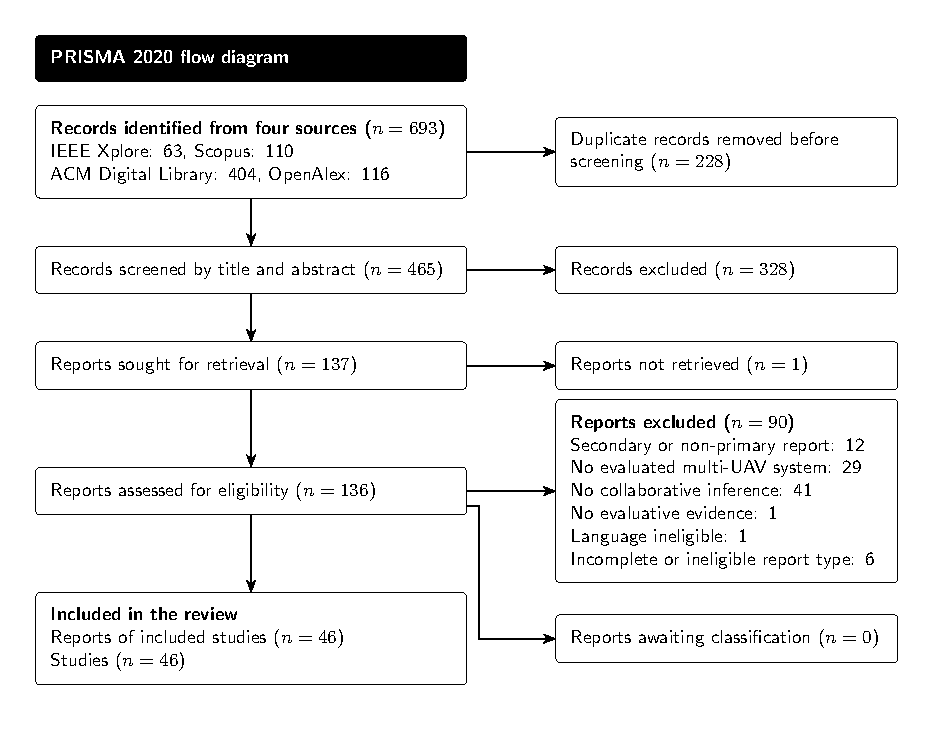
\includegraphics[width=.63\linewidth]{prisma_flow.pdf}
\caption{PRISMA 2020 selection flow. Counts distinguish records, reports, and studies.}\label{fig:flow}
\end{figure*}

\subsection{Corpus composition}
Fig.~\ref{fig:macro} summarizes year and venue, neural workloads, optimization, and evaluation. Publication year is the bibliography's citation year, which can differ from an online-first date used to decide eligibility. The 2026 column is bounded by the November cutoff and cannot establish a full-calendar-year trend. The locked corpus contains no 2021 study. A targeted backward check identified the 2021 DistInference report cited by Dhuheir et al.~\cite{R0068,dhuheir_iwcmc2021}. The candidate was absent as a record from the locked exports and was retained for a future screening update.

The workload coding includes classifiers and detectors. ASAP distributes parts of a detector workload and Orion models partitioned dense language-model inference~\cite{R0014,R0074}. NetMoE uses CIFAR-100 image classification for its representative expert-dispatch configuration in Sect. VI.B~\cite{R0118}. Mixed-family rows represent multiple evaluated families or heterogeneous learned components. LLHR evaluates LeNet and AlexNet in simulation, and the tracking handoff study uses a transformer tracker~\cite{R0082,R0292}. Generic rows retain model proxies or reference workloads when the evaluated setting lacks a concrete model family.

The modality panel separates conventional simulation from software evaluations informed by traces or device measurements. It also distinguishes software studies from bench and outdoor evaluations. See Table~\ref{tab:evaluation} for the setting of each study. In mixed evaluations, device execution and modeled wireless performance can describe different parts of one system.
\begin{table*}[!tp]
\caption{Primary inference mechanism by primary evaluation modality.}\label{tab:settings}
\centering\small\setlength{\tabcolsep}{4pt}
\begin{tabular}{@{}p{.31\linewidth}rrrrrr@{}}
\toprule
Partition or dispatch unit & Analyt. & Sim. & Trace & Bench & Outdoor & Total \\
\midrule
Sequential stages & 0 & 11 & 4 & 2 & 0 & 17 \\
Tiles, shards or tensor transport & 1 & 5 & 0 & 1 & 1 & 8 \\
Graph or early exit & 0 & 3 & 3 & 0 & 0 & 6 \\
Model or representation adaptation & 0 & 3 & 2 & 1 & 0 & 6 \\
Expert, request or state dispatch & 0 & 5 & 1 & 3 & 0 & 9 \\
Total & 1 & 27 & 10 & 7 & 1 & 46 \\
\bottomrule
\end{tabular}
\par\smallskip\raggedright Sim. denotes software evaluation. Trace denotes trace- or profile-backed evaluation. Bench includes component measurement, host emulation, and hardware-in-the-loop. Outdoor requires a multi-UAV inference evaluation.
\end{table*}

\begin{figure*}[!tp]
\centering
\resizebox{\linewidth}{!}{%
\begin{tikzpicture}[font=\fontfamily{lmss}\selectfont\footnotesize, x=1cm, y=1cm]
\definecolor{panelblue}{HTML}{236183}
\definecolor{panelteal}{HTML}{27786D}
\newcommand{\overviewbar}[5]{%
  \node[anchor=east,inner sep=1pt] at (#1,#2) {#3};
  \fill[#5] (#1+.07,#2-.12) rectangle (#1+.07+#4*.115,#2+.12);
  \node[anchor=west,inner sep=1pt] at (#1+.14+#4*.115,#2) {#4};
}
\node[anchor=west,font=\fontfamily{lmss}\selectfont\bfseries] at (0,4.15) {(a) Publication year and venue};
\node[anchor=west,font=\fontfamily{lmss}\selectfont\bfseries] at (6.9,4.15) {(b) Evaluated model families};
\node[anchor=west,font=\fontfamily{lmss}\selectfont\bfseries] at (0,-.42) {(c) Optimization approaches};
\node[anchor=west,font=\fontfamily{lmss}\selectfont\bfseries] at (6.9,-.42) {(d) Evaluation modalities};
\foreach \yr [count=\xx] in {2021,...,2026}{
  \edef\jcount{\csname yearJournal\yr\endcsname}
  \edef\ccount{\csname yearConference\yr\endcsname}
  \pgfmathsetmacro{\conferenceheight}{.16*\ccount}
  \pgfmathsetmacro{\allheight}{.16*(\jcount+\ccount)}
  \fill[panelteal!55] (\xx-.26,.7) rectangle (\xx+.26,.7+\conferenceheight);
  \fill[panelblue] (\xx-.26,.7+\conferenceheight) rectangle (\xx+.26,.7+\allheight);
  \pgfmathtruncatemacro{\total}{\jcount+\ccount}
  \node[anchor=south,inner sep=2pt] at (\xx,.7+\allheight) {\total};
  \node[anchor=north] at (\xx,.69) {\yr};
}
\draw[gray] (.60,.7)--(6.39,.7);
\fill[panelblue] (.85,-.005) rectangle (1.14,.20);
\node[anchor=west] at (1.16,.10) {Journal};
\fill[panelteal!55] (2.65,-.005) rectangle (2.94,.20);
\node[anchor=west] at (2.96,.10) {Conference};
\overviewbar{10.3}{3.57}{CNN classifiers}{\groupn{family}{cnn}}{panelblue}
\overviewbar{10.3}{3.03}{Detection}{\groupn{family}{detector}}{panelblue}
\overviewbar{10.3}{2.49}{Language models}{\groupn{family}{language}}{panelblue}
\overviewbar{10.3}{1.95}{Mixed families}{\groupn{family}{mixed}}{panelblue}
\overviewbar{10.3}{1.41}{Other named models}{\groupn{family}{other}}{panelblue}
\overviewbar{10.3}{.87}{Generic / reference}{\groupn{family}{generic}}{panelblue}
\overviewbar{3.38}{-1.01}{Mathematical}{\groupn{optimizer}{math}}{panelteal}
\overviewbar{3.38}{-1.55}{Heuristic / auction}{\groupn{optimizer}{heuristic}}{panelteal}
\overviewbar{3.38}{-2.09}{Learning-led}{\groupn{optimizer}{rl}}{panelteal}
\overviewbar{3.38}{-2.63}{Hybrid}{\groupn{optimizer}{hybrid}}{panelteal}
\overviewbar{3.38}{-3.17}{Rule / descriptive}{\groupn{optimizer}{rule}}{panelteal}
\overviewbar{10.30}{-1.01}{Analytical}{\groupn{evaluation}{analytical}}{panelteal}
\overviewbar{10.30}{-1.55}{Simulation / software}{\groupn{evaluation}{sim}}{panelteal}
\overviewbar{10.30}{-2.09}{Trace / profile simulation}{\groupn{evaluation}{trace}}{panelteal}
\overviewbar{10.30}{-2.63}{Bench / emulation / HIL}{\groupn{evaluation}{bench}}{panelteal}
\overviewbar{10.30}{-3.17}{Outdoor multi-UAV}{\groupn{evaluation}{flight}}{panelteal}
\end{tikzpicture}}

\caption{Corpus overview. The four panels assign one primary bin per study. Year conventions and coding rules are described in Sections~\ref{sec:methods} and~\ref{sec:selection}.}\label{fig:macro}
\end{figure*}


\section{Architectures, Partitioning, and Optimization}\label{sec:architecture}
\subsection{Execution topologies and architectural patterns}
\textbf{Intra-swarm peers (\groupcite{topology}{peer}).}
Peer systems keep the primary inference path inside the aerial group. Examples include choosing a neighboring UAV for a task and passing activations between stages~\cite{R0010,R0092}. Each assigned stage needs compute and a feasible path for any payload it receives. The reference-tensor study models the transport traffic incurred below that inference boundary~\cite{R0121}.

\textbf{Cluster or head--worker execution (\groupcite{topology}{cluster}).}
A coordinating role groups nodes or allocates work. In ASAP, pipeline stages span clusters and spatial subtasks are distributed inside a cluster~\cite{R0014}. Expert dispatch and redundant transformer execution track the availability of hosted experts or replicas~\cite{R0110,R0118}. These designs raise separate questions about updating the allocation after a membership change and reassigning the coordinator itself. ASAP reports rescheduling after deliberate head disconnection~\cite{R0014}.

\textbf{Air--edge or air--edge--cloud execution (\groupcite{topology}{tier}).}
These studies use an infrastructure tier or coordinate aerial edge servers with other endpoints. In one design two cuts divide a model among the vehicle, selected edge server, and optional cloud server~\cite{R0001}. Another sends a compact representation and can send additional data under a confidence rule~\cite{R0080}. If the path uses an additional tier, the transfer to that tier adds a link term. The category groups systems by functional roles, including ground clients served by aerial edge nodes and sensing UAVs using terrestrial edge nodes.

\begin{figure*}[!tp]
\centering
\resizebox{.98\linewidth}{!}{%
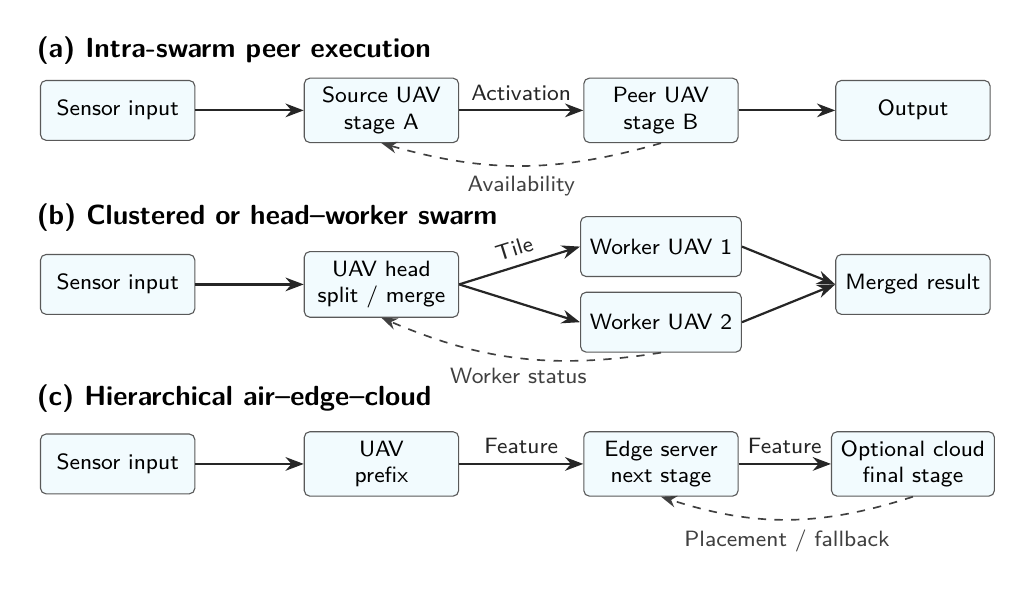
\begin{tikzpicture}[
 font=\fontfamily{lmss}\selectfont\footnotesize, >=Stealth,
 system/.style={draw=black!65, rounded corners=2pt, fill=cyan!5, align=center,
  minimum width=1.96cm, minimum height=.76cm},
 data/.style={->,thick,black!85}, control/.style={->,semithick,dashed,black!75},
 heading/.style={anchor=west,font=\fontfamily{lmss}\selectfont\bfseries}]
\node[heading] at (0,5.40) {(a) Intra-swarm peer execution};
\node[system] (sensor1) at (1.15,4.64) {Sensor input};
\node[system] (peer1) at (4.5,4.64) {Source UAV\\stage A};
\node[system] (peer2) at (8.05,4.64) {Peer UAV\\stage B};
\node[system] (output1) at (11.25,4.64) {Output};
\draw[data] (sensor1)--(peer1);
\draw[data] (peer1)--node[above]{Activation}(peer2);
\draw[data] (peer2)--(output1);
\draw[control] (peer2.south) to[bend left=16] node[below]{Availability} (peer1.south);

\node[heading] at (0,3.27) {(b) Clustered or head--worker swarm};
\node[system] (sensor2) at (1.15,2.43) {Sensor input};
\node[system] (head) at (4.5,2.43) {UAV head\\split / merge};
\node[system] (worker1) at (8.05,2.91) {Worker UAV 1};
\node[system] (worker2) at (8.05,1.95) {Worker UAV 2};
\node[system] (output2) at (11.25,2.43) {Merged result};
\draw[data] (sensor2)--(head);
\draw[data] (head.east) -- node[above,sloped]{Tile} (worker1.west);
\draw[data] (head.east) -- (worker2.west);
\draw[data] (worker1.east) -- (output2.west);
\draw[data] (worker2.east) -- (output2.west);
\draw[control] (worker2.south) to[bend left=16] node[below]{Worker status} (head.south);

\node[heading] at (0,.98) {(c) Hierarchical air--edge--cloud};
\node[system] (sensor3) at (1.15,.15) {Sensor input};
\node[system] (uav) at (4.5,.15) {UAV\\prefix};
\node[system] (edge) at (8.05,.15) {Edge server\\next stage};
\node[system] (cloud) at (11.25,.15) {Optional cloud\\final stage};
\draw[data] (sensor3)--(uav);
\draw[data] (uav)--node[above]{Feature}(edge);
\draw[data] (edge)--node[above]{Feature}(cloud);
\draw[control] (cloud.south) to[bend left=18] node[below]{Placement / fallback} (edge.south);
\end{tikzpicture}}

\caption{Illustrative execution topologies. Solid arrows show input, activation, or task data. Dashed arrows denote coordination or recovery signaling. The three patterns summarize functional roles across the corpus.}\label{fig:topologies}
\end{figure*}

\subsection{Partition and dispatch granularity}
\textbf{Sequential layers or stages (\groupcite{unit}{layer}).}
At a sequential cut the source executes a prefix and sends its activation to the next assigned device~\cite{R0010,R0092}. A multi-cut path repeats the transition. Under an ideal pipeline with independent stages and a steady backlog, first-result latency follows the full path and the steady inter-result interval is bounded below by its slowest stage. Stage profiles and link accounting are needed to evaluate an actual pipeline.

\textbf{Sub-layer, spatial, and tensor-level boundaries (\groupcite{unit}{spatial}).}
ASAP partitions spatial work across devices, and a workstation detector distributes image tiles and merges detections~\cite{R0014,R0125}. Convolutional tiles require halo data where receptive fields cross a tile boundary. Processing an overlap on two workers duplicates computation in that region. Language-model shards use different payloads and synchronization patterns~\cite{R0074}. Table~\ref{tab:architecture} labels the reference-tensor workload as transport analysis~\cite{R0121}.

\textbf{DAG and early-exit execution (\groupcite{unit}{branch}).}
A directed acyclic graph expresses which operations must finish before a dependent operation can start. An early exit omits later operations for requests meeting its exit rule~\cite{R0075}. Concurrent branches can shorten the critical path when workers and communication are available. An additional live replica consumes memory. Reliability inferred from a replica model and continuity observed after a fault require different evidence~\cite{R0110,R0121}.

\textbf{Adaptive model choice and representation changes (\groupcite{unit}{adaptive}).}
Adaptive designs vary a model, precision, or transmitted representation along with placement. An edge--cloud policy can send more data based on prediction confidence~\cite{R0080}. The reported comparison pairs accuracy with latency at specified conditions. The two policy points describe a trade-off in that setting.

\textbf{Expert, whole-request, and state dispatch (\groupcite{unit}{request}).}
A dispatcher can allocate an inference request or expert, or transfer tracker state~\cite{R0058,R0118,R0292}. For whole-request dispatch the collaboration is in orchestration across nodes. For expert dispatch the chosen destination must host the expert or provide access to it. For tracker handoff the transferred state and tracking performance define the continuity boundary. Both planning studies satisfy the request-level rule through evaluated assignments of identifiable inference work. Wang and Deng describe server-side language-model planning and on-device vision-language feedback, and compare orchestration configurations using response time and task success at the planning-system level (their Table~2)~\cite{R0223}. Xiao et al. assign planning requests across a small edge model and a large cloud model and compare model-use policies~\cite{R0145}. Omitting both in the sensitivity analysis gives 7 dispatch studies among 44, compared with 9 among 46 in the full corpus. Studies with retained numerical entries fall from 35 to 34, while all 51 matched entries remain (Supplement~S3).

\begin{figure*}[!tp]
\centering
\resizebox{\linewidth}{!}{%
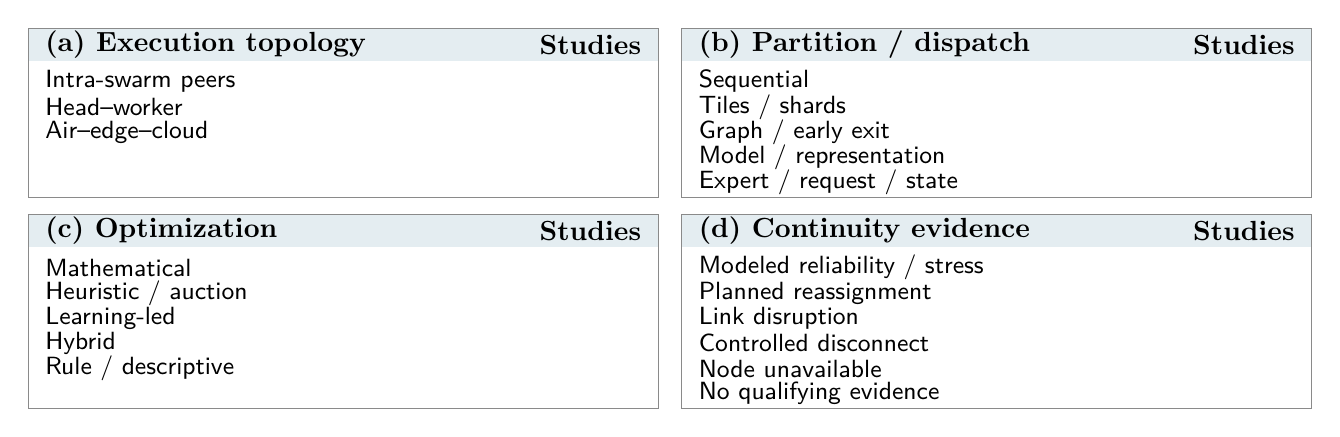
\begin{tikzpicture}[font=\fontfamily{lmss}\selectfont\small, x=1cm, y=.80cm]
\definecolor{taxheading}{HTML}{E4EDF1}
\newcommand{\taxpanel}[4]{%
  \fill[taxheading] (#1,#2) rectangle (#1+8,#2-.52);
  \draw[black!46] (#1,#2) rectangle (#1+8,#2-#3);
  \node[anchor=west,inner sep=0pt,font=\bfseries] at (#1+.21,#2-.26) {#4};
  \node[anchor=east,inner sep=0pt,font=\bfseries] at (#1+7.79,#2-.26) {Studies};
}
\newcommand{\taxrow}[5]{%
  \node[anchor=west,inner sep=0pt] at (#1+.21,#2-.45-#3*.40) {#4};
  \node[anchor=east,inner sep=0pt] at (#1+7.79,#2-.45-#3*.40) {#5};
}
\taxpanel{0}{0}{2.69}{(a) Execution topology}
\taxpanel{8.3}{0}{2.69}{(b) Partition / dispatch}
\taxpanel{0}{-2.95}{3.09}{(c) Optimization}
\taxpanel{8.3}{-2.95}{3.09}{(d) Continuity evidence}
\taxrow{0}{0}{1}{Intra-swarm peers}{\groupn{topology}{peer}}
\taxrow{0}{0}{2}{Head--worker}{\groupn{topology}{cluster}}
\taxrow{0}{0}{3}{Air--edge--cloud}{\groupn{topology}{tier}}
\taxrow{8.3}{0}{1}{Sequential}{\groupn{unit}{layer}}
\taxrow{8.3}{0}{2}{Tiles / shards}{\groupn{unit}{spatial}}
\taxrow{8.3}{0}{3}{Graph / early exit}{\groupn{unit}{branch}}
\taxrow{8.3}{0}{4}{Model / representation}{\groupn{unit}{adaptive}}
\taxrow{8.3}{0}{5}{Expert / request / state}{\groupn{unit}{request}}
\taxrow{0}{-2.95}{1}{Mathematical}{\groupn{optimizer}{math}}
\taxrow{0}{-2.95}{2}{Heuristic / auction}{\groupn{optimizer}{heuristic}}
\taxrow{0}{-2.95}{3}{Learning-led}{\groupn{optimizer}{rl}}
\taxrow{0}{-2.95}{4}{Hybrid}{\groupn{optimizer}{hybrid}}
\taxrow{0}{-2.95}{5}{Rule / descriptive}{\groupn{optimizer}{rule}}
\taxrow{8.3}{-2.95}{1}{Modeled reliability / stress}{\groupn{resilience}{analytic}}
\taxrow{8.3}{-2.95}{2}{Planned reassignment}{\groupn{resilience}{proactive}}
\taxrow{8.3}{-2.95}{3}{Link disruption}{\groupn{resilience}{link}}
\taxrow{8.3}{-2.95}{4}{Controlled disconnect}{\groupn{resilience}{bench}}
\taxrow{8.3}{-2.95}{5}{Node unavailable}{\groupn{resilience}{node}}
\taxrow{8.3}{-2.95}{6}{No qualifying evidence}{\groupn{resilience}{none}}
\end{tikzpicture}}

\caption{Technical taxonomy used in this review. Leaf counts represent primary assignments among the 46 studies in each branch. Branches describe different dimensions and each sums independently to 46.}\label{fig:taxonomy}
\end{figure*}

\subsection{A common optimization formulation}
A given inference request induces a directed graph $G=(V,E)$ whose operations or stages lie in $V$ and whose data dependencies lie in $E$. Denote a partition, exit, representation or dispatch choice by $\mathbf{x}$ and a stage-to-device or migration assignment by $\mathbf{y}$. Let $\mathbf{q}$ be UAV positions or trajectories and $\mathbf{r}=(\mathbf{f},\mathbf{p},\mathbf{b})$ denote compute rates, transmit powers, and bandwidth shares. A schematic family of objectives is
\begin{equation}
\begin{aligned}
\min_{\mathbf{x},\mathbf{y},\mathbf{q},\mathbf{r}}\quad
 &\mathbb{E}_{\omega}\bigl[\alpha_T T_{\mathrm{e2e}} + \alpha_E E_{\mathrm{tot}} \\
 &\qquad - \alpha_A A_{\mathrm{inf}} + \alpha_R C_{\mathrm{rec}}\bigr].
\end{aligned}\label{eq:objective}
\end{equation}
where $\omega$ contains workload arrivals, channel variation, and node availability. The terms are end-to-end latency, system energy, inference quality, and recovery cost. Each weight absorbs unit scaling. When the underlying metrics have different task meanings, normalization and the actual reported units must remain explicit. A recovery penalty can represent lost work or interruption cost. If recovery delay is already included in $T_{\mathrm{e2e}}$, its separate penalty must account for a distinct cost or state the intentional weighting.

A crossed dependency $e=(u,v)$ with payload $s_e(\mathbf{x})$ contributes communication delay. A first-order decomposition on the link from $i$ to $j$ is
\begin{equation}
 T_{e,ij}\approx T^{\mathrm{queue}}_{ij}
     +\frac{s_e(\mathbf{x})}{R_{ij}(\mathbf{q},\mathbf{r},\omega)}
     +T^{\mathrm{protocol}}_{ij}.
\label{eq:link}
\end{equation}
The effective rate and additive terms use a common accounting boundary. Queue and protocol terms exclude costs already folded into the rate. Serial delays add along a path. Parallel completion waits for the last required input or for a specified quorum. Early exits change which vertices execute, and autoregressive inference can repeat stage dependencies across decode steps. Provisioning a live replica adds its resource requirements at the host.

Assignment constraints connect the graph to device roles. Typical bounds concern peak working memory, energy, deadline, link feasibility, and vehicle separation. Memory includes weights and live intermediate state, with replicas counted at their actual locations. Mobility feasibility limits where nodes can move. Reliability can constrain the probability of completing before a deadline or the tolerated disruption set. Constraints need only apply to the study setting. A stationary test can set $\mathbf{q}$ exogenously. A request auction can fix the model graph and choose $\mathbf{y}$, while layer-and-hover co-design varies both placement and geometry~\cite{R0006,R0058}. In a threshold-driven transfer policy, $\mathbf{x}$ changes the payload and accuracy boundary~\cite{R0080}. Equation~\ref{eq:objective} provides a vocabulary for comparing these subproblems. It does not imply that every study measured every term.

\subsection{Optimization scopes and solution methods}
\textbf{Mathematical optimization (\groupcite{optimizer}{math}).}
Graph and resource models define the subproblem for mathematical optimization. The hover-position subproblem in the hybrid layer-cut and hover design and the language-model placement problem use different variables and feasibility constraints~\cite{R0006,R0074}. Reported solver guarantees and costs apply to their corresponding subproblem and test conditions.

\textbf{Heuristic or auction allocation (\groupcite{optimizer}{heuristic}).}
An auction can match requests and resources through bids, and a heuristic can exchange partial information about reachable workers~\cite{R0058,R0077}. An online-cost measurement should include bids, required state exchange, and schedule recomputation when they precede execution.

\textbf{Learning-led allocation (\groupcite{optimizer}{rl}).}
Learning-led examples include PPO cell/layer allocation and DQN neighbor selection~\cite{R0019,R0092}. Centralized training with decentralized execution changes which information the policy uses at dispatch~\cite{R0106}. If observation assembly and feasibility checks precede dispatch, the full online latency includes their time as well as policy evaluation.

\textbf{Hybrid search and control (\groupcite{optimizer}{hybrid}).}
Hybrid methods combine distinct solution steps. A tiered allocation design pairs PPO with continuous resource allocation~\cite{R0001}. Any resource solve or cache update on the decision path contributes to its online latency.

\textbf{System rules or descriptive models (\groupcite{optimizer}{rule}).}
Explicit deployment rules and analytical protocol models can provide evidence independently of an optimization algorithm. The container test measures prototype behavior, and the frame-delivery analysis estimates a transport boundary~\cite{R0038,R0121}. An optimality or scaling claim would require evidence for that separate question.

For RQ1 and RQ2, Tables~\ref{tab:architecture} and \ref{tab:evaluation} record what each design distributes, which variables it controls, and the conditions under which the design was tested.

For online placement, we recommend reporting the number of workers, candidate stages, communication rounds, and the timing boundary.

\begin{table*}[!tp]
\caption{Architecture, workload, partitioning, and optimization across all 46 included studies. Rows follow primary topology and year. DP means dynamic programming.}\label{tab:architecture}
\centering
\fontsize{8}{10}\selectfont\setlength{\tabcolsep}{2.5pt}\renewcommand{\arraystretch}{1.08}
\begin{tabular}{@{}Y{0.0705\linewidth}Y{0.1043\linewidth}Y{0.1589\linewidth}Y{0.1363\linewidth}Y{0.1419\linewidth}Y{0.1175\linewidth}Y{0.1307\linewidth}@{}}
\toprule
Ref. & Topology & DNN / task & Partition / dispatch & Decisions & Objective & Solver \\
\midrule
\cite{R0003}\newline\mbox{(2023)} & Intra-swarm peers & VGG-16, AlexNet, SqueezeNet & Model choice with layer placement & Model and layer assignment & Accuracy-latency utility & Genetic search \\
\cite{R0015}\newline\mbox{(2023)} & Intra-swarm peers & AlexNet, VGG-16, ResNet-152 & Intra-layer subtasks & UAV assignments per layer & Capture-to-result latency & EECIA heuristic \\
\cite{R0082}\newline\mbox{(2023)} & Intra-swarm peers & LeNet and AlexNet classification & One UAV per CNN layer; intermediate transfer & Transmit power, UAV positions, layer assignment & Latency and transmit power; rate constraint & Three mathematical subproblems; solver setup NR \\
\cite{R0010}\newline\mbox{(2024)} & Intra-swarm peers & AlexNet, GoogLeNet, VGG-16 & Per-request pipeline cuts & Layer counts on successive stages & Inference latency & Hierarchical DQN \\
\cite{R0062}\newline\mbox{(2024)} & Intra-swarm peers & Faster R-CNN video detection & Pipelined submodels & Partition and remaining-node assignment & Inference rate and continuity & Adaptive OODA scheduler \\
\cite{R0073}\newline\mbox{(2024)} & Intra-swarm peers & AlexNet, VGG-16, YOLO & CNN layers & Layer allocation and UAV operability & End-to-end latency & ILP formulation; PPO policy \\
\cite{R0006}\newline\mbox{(2025)} & Intra-swarm peers & Synthetic layered detection DNN & Layer assignment & Hover positions and layer placement & Pipeline completion time & Alternating DP and continuous placement \\
\cite{R0059}\newline\mbox{(2025)} & Intra-swarm peers & AlexNet and VGG-16 streams & Model switching and layer cuts & Models and layer assignments & Aggregate delay at accuracy target & Horizon switching plus MADDPG \\
\cite{R0068}\newline\mbox{(2025)} & Intra-swarm peers & LeNet and AlexNet classification & Layer-wise split & Layer placement and power & Latency and transmit power & Offline allocation plus multi-agent meta-RL \\
\cite{R0292}\newline\mbox{(2025)} & Intra-swarm peers & OSTrack marine video tracking & Tracking-state handoff & Tracker and matching configuration & Persistent monitoring through handoff & Protocol and component tuning \\
\cite{R0074}\newline\mbox{(2026)} & Intra-swarm peers & Llama-2 multisensor logs & Layer and sequence partitions & Stage mapping and token splits & Bottleneck prefill latency & State-compressed and min-max DP \\
\cite{R0077}\newline\mbox{(2026)} & Intra-swarm peers & Modeled layered inference graph & Distributed graph with early exits & Offload threshold and exit & Congestion and completion & Capacity diffusion and threshold rules \\
\cite{R0092}\newline\mbox{(2026)} & Intra-swarm peers & VGG and other vision models & Two-UAV mini-batch pipeline & Peer and cut selection & Deadline and energy trade-offs & Pareto shortlist and DQN \\
\cite{R0121}\newline\mbox{(2026)} & Intra-swarm peers & Reference detector-like activation tensor & Activation transport and fragmentation & Encoding and protocol representation & Analytical latency and traffic & Link-layer analytical model \\
\cite{R0029}\newline\mbox{(2022)} & Cluster or head--worker & AlexNet, VGG-19, GoogLeNet, ResNet-101 & DAG layer replicas & Layer-to-UAV replica mapping & Energy at deadline and reliability limits & DQN with penalties \\
\cite{R0019}\newline\mbox{(2023)} & Cluster or head--worker & LeNet, AlexNet, VGG-16 & CNN layers & Grid position and layer allocation & Image decision delay & PPO \\
\cite{R0043}\newline\mbox{(2023)} & Cluster or head--worker & NiN, VGG-16, AlexNet, ResNet-18 & Overlapping spatial sub-blocks & Fusion depth and UAV coalition & Total inference time & Fine partition plus genetic matching \\
\cite{R0014}\newline\mbox{(2024)} & Cluster or head--worker & Six CNNs; video & Spatial shards within layer pipelines & Cluster and worker assignment & Latency and load balance & ASAP scheduling and profiling \\
\cite{R0022}\newline\mbox{(2025)} & Cluster or head--worker & Branchy AlexNet recognition & Early exit plus layer cuts & Exit choice and model allocation & Accuracy, delay and energy utility & Option-Critic hierarchical RL \\
\cite{R0083}\newline\mbox{(2025)} & Cluster or head--worker & AlexNet and VGG-19 & Containerized partitions & Container placement and resources & Normalized delay and energy & MILP with constructive approximation \\
\cite{R0106}\newline\mbox{(2025)} & Cluster or head--worker & Layered target-awareness model & Sequential inference portions & Partition and multi-agent coordination & Continuity and inference quality & Split DRL with decentralized execution \\
\cite{R0223}\newline\mbox{(2025)} & Cluster or head--worker & LLM coordination and multimodal feedback & Task-graph assignment & Task ordering and collaborative policy & Response and completion & Task-graph rules plus PPO variant \\
\cite{R0002}\newline\mbox{(2026)} & Cluster or head--worker & ResNet-18 classification & Two dependent modules & Cross-swarm and service migration & Weighted migration time and energy & Predictive migration heuristic \\
\bottomrule
\end{tabular}
\end{table*}

\begin{table*}[!tp]
\centering\footnotesize \MakeUppercase{\tablename}\ \ref{tab:architecture} (continued)\par\smallskip
\centering
\fontsize{8}{10}\selectfont\setlength{\tabcolsep}{2.5pt}\renewcommand{\arraystretch}{1.08}
\begin{tabular}{@{}Y{0.0705\linewidth}Y{0.1043\linewidth}Y{0.1589\linewidth}Y{0.1363\linewidth}Y{0.1419\linewidth}Y{0.1175\linewidth}Y{0.1307\linewidth}@{}}
\toprule
Ref. & Topology & DNN / task & Partition / dispatch & Decisions & Objective & Solver \\
\midrule
\cite{R0048}\newline\mbox{(2026)} & Cluster or head--worker & YOLOv3-tiny video analytics & Classifier-level DAG & Position and graph scheduling & Inference latency & GA\allowbreak{}/DP or MAPPO\allowbreak{}/DAG scheduling \\
\cite{R0075}\newline\mbox{(2026)} & Cluster or head--worker & Early-exit CNN classification & Feature exchange and branch assignment & Confidence- and cost-aware exit routing & Accuracy and inference cost & Frozen LinUCB exit router \\
\cite{R0095}\newline\mbox{(2026)} & Cluster or head--worker & ResNet-50, MobileNetV3 and BERT & Macro-block pipeline and cache & Cuts, displacement and cache policy & Delay and completion & PPO plus cache heuristic \\
\cite{R0110}\newline\mbox{(2026)} & Cluster or head--worker & Llama-2 transformer inference & Redundant feed-forward shards & Replica deployment and selective activation & Latency and continuity under resource limits & Offline placement and online scheduling \\
\cite{R0118}\newline\mbox{(2026)} & Cluster or head--worker & CIFAR-100 image classification (Sect. VI.B configuration) & Expert dispatch & Expert placement, selection and motion & Latency and communication constraints & Learned orchestration and control \\
\cite{R0125}\newline\mbox{(2026)} & Cluster or head--worker & YOLO11m ONNX video detection & Overlapping frame tiles & Frame regions and worker threads & Throughput and latency & Worker allocation and tile adaptation \\
\cite{R0089}\newline\mbox{(2023)} & Air--edge or air--edge--cloud & Branchy ResNet; CIFAR-10 & Early exit and feature offload & Upload priority and queue balancing & Delay and load & Priority queues and load balancing \\
\cite{R0044}\newline\mbox{(2024)} & Air--edge or air--edge--cloud & AlexNet and TinyYOLOv2 among tested models & Row-wise activation tiles & Partition, power and offloading & Reliable latency\allowbreak{}/energy trade-off & Subgradient and KKT updates \\
\cite{R0038}\newline\mbox{(2025)} & Air--edge or air--edge--cloud & TensorFlow CNN classification & Containerized CNN stages & Container placement constraints & Pipeline continuity & Docker Swarm placement \\
\cite{R0064}\newline\mbox{(2025)} & Air--edge or air--edge--cloud & Frame-oriented sensing and inference & Frame sampling and binary offload & 3D motion, sampling, offload & Delay at sensing and accuracy constraints & Hybrid-action MAPPO \\
\cite{R0071}\newline\mbox{(2025)} & Air--edge or air--edge--cloud & ResNet-18 recognition & Single cut at macro-block & Split, radio, CPU and offload & Weighted delay and energy & LSTM-enhanced multi-agent policy \\
\cite{R0080}\newline\mbox{(2025)} & Air--edge or air--edge--cloud & ResNet-18 and ResNet-101; CIFAR-10 & Feature-first and optional quantized raw input & Thresholds and input quantization & Accuracy under shared bandwidth & Alternating optimization \\
\cite{R0090}\newline\mbox{(2025)} & Air--edge or air--edge--cloud & Agricultural CNN inference & Local inference task assignment & Coverage and energy-aware allocation & Coverage and task continuity & Redundancy and consensus design \\
\cite{R0145}\newline\mbox{(2025)} & Air--edge or air--edge--cloud & Language-model industrial planning requests & Small-edge and large-cloud requests & Model roles and selective replay & Completion, runtime and cost & System rules and model selection \\
\cite{R0001}\newline\mbox{(2026)} & Air--edge or air--edge--cloud & Generic layered DNN proxy & Two cuts across three tiers & Cuts, edge selection, compute and radio & Latency and resources & PPO plus convex allocation \\
\cite{R0009}\newline\mbox{(2026)} & Air--edge or air--edge--cloud & ResNet-34, VGG-16, AlexNet & Ground-to-UAV layer cut & Cut, matching, motion, radio and compute & Latency and energy & Partition search, matching and DRL \\
\cite{R0036}\newline\mbox{(2026)} & Air--edge or air--edge--cloud & YOLOv5 pedestrian video & Configured stream or chunk & Stream, resolution and frame rate & Weighted coverage at accuracy and capacity limits & Profile plus greedy local search \\
\cite{R0045}\newline\mbox{(2026)} & Air--edge or air--edge--cloud & AlexNet, VGG-16, VGG-13 & Binary layer split, with migration & Matching, split, motion, compute & Delay and energy under service constraints & SAC plus convex allocation \\
\cite{R0054}\newline\mbox{(2026)} & Air--edge or air--edge--cloud & Profiled semantic inference & Tier cuts and feature quantization & Heading, resource and feature bit width & Composite sensing, inference and resource cost & Graph-assisted policy and deterministic allocation \\
\cite{R0058}\newline\mbox{(2026)} & Air--edge or air--edge--cloud & ResNet-18; CIFAR-10 requests & Indivisible requests & Bids, server matching, local execution & Aggregate auction utility & Distributed auction \\
\cite{R0063}\newline\mbox{(2026)} & Air--edge or air--edge--cloud & Distributed language-model inference & Tiered draft and verification & Model roles and execution policy & Inference and coordination performance & Role-decoupled multi-agent RL \\
\cite{R0107}\newline\mbox{(2026)} & Air--edge or air--edge--cloud & Semantic fusion for visual question answering & Distributed representations and semantic granularity & Fusion weights and granularity & Task quality under communication limit & Two-stage reinforcement learner \\
\cite{R0137}\newline\mbox{(2026)} & Air--edge or air--edge--cloud & Traffic video detection CNNs & Local or edge inference per task & Placement, input and model settings & Accuracy and modeled reliability & Multi-agent policy \\
\bottomrule
\end{tabular}
\end{table*}


\section{Evaluation, Resilience, and Evidence Appraisal}\label{sec:evaluation}
\subsection{Evaluation modalities, wireless assumptions, and mobility}
\textbf{Analytical configurations (\groupcite{evaluation}{analytical}).}
The reference-tensor analysis derives serialization and intact-delivery estimates from fragmentation and frame-loss assumptions~\cite{R0121}. The outputs are analytical estimates for a specified payload and delivery rule.

\textbf{Software simulation (\groupcite{evaluation}{sim}).}
The simulations include examples of modeled computation and communication under fixed-rate or distance-dependent links~\cite{R0015,R0022}. Such results are conditional on the implemented assumptions. A transmitter-rate equation alone specifies service rate. Competition for that service requires a separately specified sharing or queueing rule.

\textbf{Trace- or profile-backed simulation (\groupcite{evaluation}{trace}).}
Mid-Air trajectories provide simulated geometry in two studies~\cite{R0003,R0010}. CIDER uses Jetson TX2 device profiles and modeled communication~\cite{R0075}. A replayed trajectory supplies positions, and a device profile supplies compute measurements under its stated conditions. An airborne throughput claim would require throughput observations from the relevant deployment.

\textbf{Bench, emulation, or hardware-in-the-loop evaluations (\groupcite{evaluation}{bench}).}
The container recovery study exercises deployed software on a stationary testbed~\cite{R0038}. The frame-tiling study implements HTTP transfer and measures workstation throughput~\cite{R0125}. The tracker study reports a hardware-in-the-loop evaluation of handoff and tracking~\cite{R0292}. Each supports behavior under its stated evaluation conditions.

\textbf{Outdoor multi-UAV inference evaluation (\groupcite{evaluation}{flight}).}
ASAP reports an outdoor five-UAV setting and an indoor embedded deployment. Its disconnection result is separately located. Treating the outdoor result as evidence of an outdoor disconnect test would attach the wrong conditions to the claim.

Network assumptions include constant rate, distance-dependent loss, probabilistic line of sight, 802.11s packet drops, and frame fragmentation~\cite{R0015,R0022,R0073,R0083,R0121}. The extraction records these at their respective levels of modeling. Mobility can enter as static geometry, simulated or replayed trajectories, or actual flight~\cite{R0003,R0014,R0074}. Table~\ref{tab:evaluation} records the deployment and network or mobility conditions documented for each study.

NetMoE compares expert and layer-wise configurations with the same centralized planner in its simulation~\cite{R0118}. The workstation comparison increases the total nominal worker thread allocation when it adds workers~\cite{R0125}. Outcomes describe the tested configurations. An isolated effect would require holding other relevant workload and resource conditions fixed. For RQ3, software and trace-backed evaluations account for 37 of 46 studies (Fig.~\ref{fig:macro}). Hardware and flight claims therefore depend on the setup of each reported experiment.

\subsection{Continuity and fault-recovery evidence}
\textbf{Modeled reliability or stress (\groupcite{resilience}{analytic}).}
The frame-delivery study provides an analytical result without simulation or empirical validation. The attribution of its probability input remains unresolved~\cite{R0121}. Orion varies bandwidth in simulation~\cite{R0074}. Dhuheir et al. vary the active set from three to four and then two UAVs in simulation. The learning reward reconverges after changes in membership in their Fig.~19. This supports modeled policy adaptation under membership changes. Transfer of an in-progress request or state, and time to first correct resumed inference output, are unreported for that experiment~\cite{R0019}.

\textbf{Planned reassignment (\groupcite{resilience}{proactive}).}
Meng et al. model service migration triggered by load or energy thresholds~\cite{R0045}. Transformer tracking evaluates planned state handoff in hardware-in-the-loop~\cite{R0292}. A planned handoff with access to outgoing state describes a separate condition from abrupt worker disappearance.

\textbf{Link disruption or tier fallback (\groupcite{resilience}{link}).}
The auction study describes retries, buffering, and local execution under short contacts~\cite{R0058}. DDCI evaluates resource-aware choices among candidate peers and local execution under dynamic links~\cite{R0092}. A collaboration model sends an incomplete task to a base station for reprocessing after return-data failure~\cite{R0044}. These evaluations report the modeled response or connectivity sensitivity without phase-level fallback timing.

\textbf{Controlled disconnection (\groupcite{resilience}{bench}).}
In the Docker Swarm prototype, input continued while a dependent stage waited, and computation resumed from an intermediate result in Redis~\cite{R0038}. A separate test disabled a device's communication program and reassigned work. ASAP reports rescheduling latency after deliberate head disconnection~\cite{R0062,R0014}. Rescheduling time and time to the first correct resumed output are separate measures.

\textbf{Node unavailability with recovery or completion evidence (\groupcite{resilience}{node}).}
Predictive migration includes modeled random UAV failures, and other studies vary available nodes or model selectively activated replicas~\cite{R0002,R0073,R0106,R0110}. The observed quantities are specific to the stress and available outputs. Phase-resolved recovery and validation during flight require separate evidence.

\textbf{No qualifying continuity evidence (\groupcite{resilience}{none}).}
These studies inform architecture, optimization or evaluation, with no qualifying disruption-and-response evidence in the accepted extraction. Variable channels, normal queue dynamics, and a backup described without evaluation should not be read as measured fault recovery. Table~\ref{tab:evaluation} preserves relevant partial descriptions even where the aggregate class records no recovery evidence. Fig.~\ref{fig:taxonomy} shows the distribution across evidence categories. The counts use all 46 studies, with one primary category per study. For RQ4, claims about continuing inference depend on which event was evaluated and which response was measured. A recovery-time claim needs a defined start event and a measured endpoint, such as the first correct resumed output.
\begin{table*}[!tp]
\caption{Evaluation modality, network and mobility, resilience, and artifact reporting for all 46 studies. Artifact status records the D09 judgment. NR denotes not reported in the accepted evidence.}\label{tab:evaluation}
\centering
\fontsize{8}{10}\selectfont\setlength{\tabcolsep}{2.5pt}\renewcommand{\arraystretch}{1.08}
\begin{tabular}{@{}Y{0.0705\linewidth}Y{0.1090\linewidth}Y{0.1598\linewidth}Y{0.1532\linewidth}Y{0.1466\linewidth}Y{0.1438\linewidth}Y{0.0724\linewidth}@{}}
\toprule
Ref. & Modality & Hardware / simulator & Network / mobility & Disruption / failure & Continuity action & Code / data \\
\midrule
\cite{R0003}\newline\mbox{(2023)} & Trace or profile sim. & Mid-Air-driven simulation & Trace-derived rate variation & NR & NR & NR \\
\cite{R0015}\newline\mbox{(2023)} & Simulation & Simulated embedded devices & Fixed per-request rate; full reachability & NR & NR & NR \\
\cite{R0082}\newline\mbox{(2023)} & Simulation & Simulation with Raspberry Pi-class resource parameters & Same-altitude grid; distance-dependent data rate & No isolated outage test reported & Capacity-based delegation described & NR \\
\cite{R0010}\newline\mbox{(2024)} & Trace or profile sim. & Mid-Air-driven simulation & Trace-derived inter-UAV rates & NR & NR & NR \\
\cite{R0062}\newline\mbox{(2024)} & Bench or emulation & Four heterogeneous Jetson-equipped units & Airborne modules; flight fault test unestablished & Radio software disabled on one UAV & Reallocate unfinished stages & NR \\
\cite{R0073}\newline\mbox{(2024)} & Simulation & Numerical simulation & Operability state; cell-based placement & Up to two modeled inoperable UAVs & Reassign layers & NR \\
\cite{R0006}\newline\mbox{(2025)} & Simulation & Synthetic layer profiles; numerical simulation & Planar hover; distance-based rate & NR & NR & NR \\
\cite{R0059}\newline\mbox{(2025)} & Trace or profile sim. & Mid-Air traces and embedded specs & Predetermined swarm trajectory & NR & NR & NR \\
\cite{R0068}\newline\mbox{(2025)} & Simulation & Python and TensorFlow simulation & Changing membership and return on depletion & Energy depletion and joins\allowbreak{}/leaves & Delegate work to another UAV & NR \\
\cite{R0292}\newline\mbox{(2025)} & Bench or emulation & Recorded marine video and hardware-in-loop & Wi-Fi transfer; logged footage & Planned operational handoff & Transfer tracking state & NR \\
\cite{R0074}\newline\mbox{(2026)} & Simulation & Python LLM simulator with profiles & Modeled bandwidth jitter and compute variation & Rate and compute perturbations & Sensitivity, not fault recovery & Partial \\
\cite{R0077}\newline\mbox{(2026)} & Simulation & Layered-graph simulator & Circular paths and modeled LoS neighbors & Physical node failure NR & NR & NR \\
\cite{R0092}\newline\mbox{(2026)} & Trace or profile sim. & Profile-grounded Gymnasium simulation & Modeled Wi-Fi and changing links & Peer leaves communication range & Reassign or recompute locally & Yes \\
\cite{R0121}\newline\mbox{(2026)} & Analytical & Analytical calculations only & Modeled 802.11 and frame loss & Analytical results, no simulation or empirical validation & Probability-input attribution unresolved & NR \\
\cite{R0029}\newline\mbox{(2022)} & Trace or profile sim. & Numerical simulation with layer profiles & Poisson transient node\allowbreak{}/link fault model & Probabilistic transient failure & Active replication & NR \\
\cite{R0019}\newline\mbox{(2023)} & Simulation & Grid and arrival simulation & Grid motion; no Doppler evaluation & Simulated active count changes (3 to 4 to 2) & Learning reward re-converges; handoff and resumed output unreported & NR \\
\cite{R0043}\newline\mbox{(2023)} & Simulation & SeaShip simulation & Fixed system bandwidth & NR & NR & NR \\
\cite{R0014}\newline\mbox{(2024)} & Outdoor flight & Indoor embedded test plus five-UAV outdoor run & Indoor Wi-Fi; outdoor ad hoc radios & Deliberate head disconnection; outdoor status unestablished & Reschedule surviving devices & Partial \\
\cite{R0022}\newline\mbox{(2025)} & Simulation & Serverless swarm simulation & Distance loss and complex-normal coefficient & NR & NR & NR \\
\cite{R0083}\newline\mbox{(2025)} & Simulation & Python network and energy simulation & 802.11s loss model; group mobility & Battery heterogeneity & Fault recovery NR & NR \\
\cite{R0106}\newline\mbox{(2025)} & Simulation & Python\allowbreak{}/PyTorch simulation & Modeled network; variable participation & Simulated loss of participating nodes & Continue on available nodes & NR \\
\cite{R0223}\newline\mbox{(2025)} & Simulation & AirSim and MATLAB software & Simulated obstacles and coordination & Airborne outage NR & NR & NR \\
\cite{R0002}\newline\mbox{(2026)} & Simulation & PC simulation with embedded parameters & Cross-swarm movement; battery return & Random node unavailability in simulation & Predictive and recovery migration & NR \\
\bottomrule
\end{tabular}
\end{table*}

\begin{table*}[!tp]
\centering\footnotesize \MakeUppercase{\tablename}\ \ref{tab:evaluation} (continued)\par\smallskip
\centering
\fontsize{8}{10}\selectfont\setlength{\tabcolsep}{2.5pt}\renewcommand{\arraystretch}{1.08}
\begin{tabular}{@{}Y{0.0705\linewidth}Y{0.1090\linewidth}Y{0.1598\linewidth}Y{0.1532\linewidth}Y{0.1466\linewidth}Y{0.1438\linewidth}Y{0.0724\linewidth}@{}}
\toprule
Ref. & Modality & Hardware / simulator & Network / mobility & Disruption / failure & Continuity action & Code / data \\
\midrule
\cite{R0048}\newline\mbox{(2026)} & Trace or profile sim. & Server simulation with measured embedded profiles & Fixed hover; LoS attenuation & NR & NR & NR \\
\cite{R0075}\newline\mbox{(2026)} & Trace or profile sim. & Jetson TX2 profiles; modeled links & Rate sweeps and waiting & NR & NR & NR \\
\cite{R0095}\newline\mbox{(2026)} & Simulation & RTX 4060 workstation simulation & Planar motion with minimum separation & Backup proposed; test NR & Backup controller described & NR \\
\cite{R0110}\newline\mbox{(2026)} & Simulation & Discrete-event simulator & 3GPP-informed channel; mobility stress & Modeled worker and leader disruptions & Replica activation and leader recovery & NR \\
\cite{R0118}\newline\mbox{(2026)} & Simulation & Software swarm simulation & Modeled mobility and connectivity stress & Connectivity stress sensitivity & Expert-routing response; recovery phases NR & Yes \\
\cite{R0125}\newline\mbox{(2026)} & Bench or emulation & AMD workstation with emulated workers & HTTP\allowbreak{}/JPEG; no measured airborne channel & Thread-budget changes; link failure test NR & Stateless replacement described & NR \\
\cite{R0089}\newline\mbox{(2023)} & Simulation & PyTorch and software simulation & Modeled network; motion NR & NR & NR & No \\
\cite{R0044}\newline\mbox{(2024)} & Simulation & Numerical MEC simulation & Unreliable links; circular UAV motion & Failed return data modeled & Reprocess whole task at ground BS & NR \\
\cite{R0038}\newline\mbox{(2025)} & Bench or emulation & Two computers and two Raspberry Pi 5 devices & Bench network; UAV motion absent & Deliberate device disconnection & Redeploy and resume from Redis & NR \\
\cite{R0064}\newline\mbox{(2025)} & Simulation & Air-ground numerical simulation & 3D trajectory; congestion loss omitted & NR & NR & NR \\
\cite{R0071}\newline\mbox{(2025)} & Simulation & Custom simulation & Generated mobility and energy harvesting & Depletion represented in model & Recovery NR & NR \\
\cite{R0080}\newline\mbox{(2025)} & Simulation & Synthesized data splits; modeled uplink & Spectral efficiency; trajectories NR & NR & NR & NR \\
\cite{R0090}\newline\mbox{(2025)} & Bench or emulation & Software stack and author-reported hardware prototype & Modeled loss; LoRaWAN ground sensing & Reported dropout; test modality unclear per outcome & Redundant reassignment described & NR \\
\cite{R0145}\newline\mbox{(2025)} & Simulation & Lab server; generated scenarios & Modeled motion and communication & Inference errors; outage NR & Replay revises earlier decisions & NR \\
\cite{R0001}\newline\mbox{(2026)} & Trace or profile sim. & Delivery and base-station data; simulation & Distance-dependent air-ground links & NR & NR & NR \\
\cite{R0009}\newline\mbox{(2026)} & Trace or profile sim. & Profile-driven simulation & Moving aerial MEC; LoS path loss & NR & NR & NR \\
\cite{R0036}\newline\mbox{(2026)} & Trace or profile sim. & Ground-view ETH video; simulation & Shared bandwidth; synthetic surveillance positions & NR & NR & NR \\
\cite{R0045}\newline\mbox{(2026)} & Simulation & Python, PyTorch and CVX & 3D motion; link and compute model & Energy or load threshold & Migrate inference service & NR \\
\cite{R0054}\newline\mbox{(2026)} & Simulation & Multi-UAV ISCC simulation & Heading-sensitive STAR-RIS model & NR & NR & NR \\
\cite{R0058}\newline\mbox{(2026)} & Simulation & Dynamic-edge simulation & Speed alters contact time & Short contacts; fallback described & Retry, buffer or simplified local inference & NR \\
\cite{R0063}\newline\mbox{(2026)} & Bench or emulation & Component profile plus software evaluation & Modeled intermittent links and delay & Simulated connectivity degradation & Tier fallback described & Partial \\
\cite{R0107}\newline\mbox{(2026)} & Simulation & RTX workstation; modeled edge nodes & Variable channel; route NR & NR & NR & NR \\
\cite{R0137}\newline\mbox{(2026)} & Bench or emulation & Physical profiling\allowbreak{}/deployment plus modeled links & Probabilistic path loss and disturbance model & Modeled compute\allowbreak{}/link unreliability & Reliability-aware configuration & NR \\
\bottomrule
\end{tabular}
\end{table*}


\subsection{Condition-specific quantitative comparisons}
The uniform reread retained 97 entries from 35 of 46 studies, including 51 matched entries from 23 studies and 46 descriptive entries. Eleven studies had plot-only outcomes under the extraction rule. LLHR contributes to this group because its latency and transmit-power results are shown as curves~\cite{R0082}. Table~\ref{tab:coverage} shows coverage by mechanism. For layers or stages, Table~\ref{tab:settings} records 15 of 17 studies in simulation or trace-backed evaluation, two in bench evaluation, and zero in outdoor evaluation. Table~\ref{tab:outcomes} selects nine illustrative within-study contrasts and retains their original workloads, units, and measurement boundaries.

In the 100 Mb/s edge--cloud test, the proposed policy had higher mean top-1 accuracy and mean latency than GSUP with the ResNet-18/101 pair. The intervals are 95\% Student-$t$ confidence intervals across three seeds. The separate 100 MHz sweep at 20 UAVs reports an accuracy advantage of 0.9\% over GSUP and 1.5\% over Raw-Only in the prose. The difference scale and the GSUP/GDUP legend discrepancy remain unresolved~\cite{R0080}.\par In the two-UAV VGG-16 simulation, DDCI had higher mean deadline satisfaction than Comm-Min. System-total compute and communication energy was $1.477\pm0.054$ Wh for DDCI and $1.502\pm0.048$ Wh for Comm-Min (mean $\pm$ SD, 30 common-seed episodes)~\cite{R0092}.

In Orion's parameterized simulation for Llama-2 7B at a 64-token input, distributed prefill is faster than the cloud-assisted configuration and slower than the single-device configuration, where the model fits~\cite{R0074}. These are prefill times for that setup. For Llama-2 70B, RDI-LLM and Orion-DP report approximately 0.8 and 0.3~s per token over the 30 and 22 missions they completed, respectively, from 30 seeded missions per method~\cite{R0110}. The per-token averages condition on different completed sets. CIDER's comparison covers a routing boundary with profiled computation and modeled communication~\cite{R0075}.

ASAP reports seconds per task over a sequence in its indoor scale test~\cite{R0014}. The workstation study reports 12.8 FPS with two workers at four threads each versus 6.9 FPS with one four-thread worker (1.85$\times$ as reported)~\cite{R0125}. A controlled prototype continued at a lower frame rate after one device became unavailable~\cite{R0062}.\par SAC$^2$ reports 22\% greater accumulated surveillance coverage than Random-to-upload at 20 Mb/s~\cite{R0036}. AeroAgriNet's Figure 5 labels 91\% task completion at 20 UAVs. The prose claim of throughput above 90\% remains unresolved~\cite{R0090}.\par Xiao et al. report benchmark reference time to first token (TTFT) of 0.68 and 0.19 s and time per output token (TPOT) of $1/53$ and $1/246$ s for DeepSeek-R1-Distill-Llama-8B and LLaMA-3.2-3B, respectively. Attribution to local measurement remains unresolved~\cite{R0145}. For RQ5, these measurements support comparisons within the stated setups. Differences in workloads, compute budgets, and outcome boundaries limit comparisons across studies.
\begin{table*}[!tp]
\caption{Coverage of retained numerical outcomes by primary inference mechanism.}\label{tab:coverage}
\centering\small\setlength{\tabcolsep}{4pt}
\begin{tabular*}{.92\linewidth}{@{\extracolsep{\fill}}p{.34\linewidth}rrrrr@{}}
\toprule
Partition or dispatch unit & Studies & Verified & Plot only & Unresolved & Entries \\
\midrule
Sequential stages & 17 & 11 & 6 & 0 & 31 \\
Tiles, shards or tensor transport & 8 & 6 & 2 & 0 & 18 \\
Graph or early exit & 6 & 4 & 2 & 0 & 13 \\
Model or representation adaptation & 6 & 6 & 0 & 0 & 13 \\
Expert, request or state dispatch & 9 & 8 & 1 & 0 & 22 \\
Total & 46 & 35 & 11 & 0 & 97 \\
\bottomrule
\end{tabular*}
\par\smallskip\raggedright The first four numeric columns count studies. Entries counts matched or descriptive results. The extraction rule retains explicit results with interpretable conditions.
\end{table*}

\begin{table*}[!tp]
\caption{Verified within-study contrasts. Values are proposed/configuration A versus comparator/configuration B. CI denotes 95\% Student-$t$ confidence interval half-width. A plain value preserves a reported point estimate or summary. Approximate values retain the approximation mark.}\label{tab:outcomes}
\centering
\fontsize{8}{10}\selectfont\setlength{\tabcolsep}{2.5pt}\renewcommand{\arraystretch}{1.22}
\begin{tabular}{@{}Y{0.0602\linewidth}Y{0.1485\linewidth}Y{0.0968\linewidth}Y{0.0968\linewidth}Y{0.0884\linewidth}Y{0.1147\linewidth}Y{0.2529\linewidth}@{}}
\toprule
Study & Workload / setup & Method A & Baseline B & Metric & Values A / B & Conditions and locator \\
\midrule
\cite{R0080} & CIFAR-10, edge and cloud & Proposed policy & GSUP & Top-1 (\%) & \mbox{$90.4\pm0.5$ /}\newline\mbox{$89.5\pm0.5$} & ResNet-18/101, 100 Mb/s, three seeds, \mbox{mean $\pm$ CI}, p. 5, Table I \\
\cite{R0080} & Same model and data pair & Proposed policy & GSUP & Latency (ms) & $120\pm3$ / $117\pm3$ & Same condition and uncertainty; edge, transfer and cloud, p. 5, Table I \\
\cite{R0092} & VGG-16, two UAVs in simulation & DDCI & Comm-Min & Deadline success (\%) & $71.6\pm3.4$ / $64.4\pm4.3$ & \mbox{Mean $\pm$ SD} over 30 common-seed episodes; all arrivals, p. 13, Table V \\
\cite{R0075} & CIFAR-10, profiled and modeled links & CIDER & Full Final Exit & Compute + radio (ms) & 26.85 / 38.81 & Routing boundary only; frozen test router, p. 10, Table III \\
\cite{R0074} & Llama-2 7B FP16, 64 tokens & Orion & Cloud-Edge-Opt & Prefill (ms) & 8,864 / 46,522 & Simulated four-node case, 1,000 Mb/s inter-UAV, 200 Mb/s air--ground, p. 16, Sect. 4.2 and Fig. 4 \\
\cite{R0074} & Same parameterized simulation & Orion & Edge-Solo & Prefill (ms) & 8,864 / 8,047 & Same workload; single-device fit in this setting, p. 16, Sect. 4.2 and Fig. 4 \\
\cite{R0014} & ResNet-152, 720 by 1280 video & ASAP, 20 devices & ASAP, four devices & Task sequence (s/task) & 1.32 / 2.32 & Indoor devices; span of 100 tasks divided by 100, p. 12, Table III \\
\cite{R0062} & Faster R-CNN stream, embedded prototype & Three participating UAVs & Four participating UAVs & Rate (fps) & $\sim$2 / $\sim$3 & Stages reallocated after disabling device communication, p. 6, UAV unavailability test \\
\cite{R0125} & YOLO11m frame detection & Four workers & One worker & Rate (fps) & 22.4 / 6.9 & Four threads per worker; total worker thread allocations are 16 and 4, p. 3, Table I and Sect. IV.B \\
\bottomrule
\end{tabular}
\end{table*}


\subsection{Ten-domain appraisal and reproducibility}
Table~\ref{tab:appraisal} and Fig.~\ref{fig:appraisalbar} record 45/46 affirmative ratings for question and system-model clarity. Ratings were partial for configuration reproducibility in 42/46, baseline comparability in 40/46, and network and mobility realism in 43/46. D06 received 41 partial ratings. Li et al. vary request and UAV counts~\cite{R0003}, and Xiao et al. compare 20 generated scenarios~\cite{R0145}. Both studies leave independent repeats and within-setting dispersion unreported. Artifact availability was undocumented in 40/46 assessed reports, including access to study-specific code or test video within the workstation study PDF~\cite{R0125}.

The appraisal suggests concrete reporting checks. Specify data versions, splits, seeds, and configuration for reproduction. For comparisons, record resolution, precision, batch size, and thread budget where applicable. For wireless modeling, state whether spatial geometry, queueing, interfering traffic, and retransmissions are represented. Archive the configuration and orchestration needed to repeat execution.

\begin{table}[!t]
\caption{Ten-domain engineering appraisal. Each row has 46 judgments. No included report received N/A in these domains.}\label{tab:appraisal}
\centering\footnotesize\setlength{\tabcolsep}{2pt}
\begin{tabular*}{\columnwidth}{@{\extracolsep{\fill}}Y{.41\linewidth}rrrrr@{}}
\toprule
Domain & Yes & Partial & Not reported & No & Yes (\%) \\
\midrule
\technicalappraisalrows
\bottomrule
\end{tabular*}
\end{table}

\begin{figure*}[!tp]
\centering
\resizebox{.97\linewidth}{!}{%
\begin{tikzpicture}[font=\footnotesize\fontfamily{lmss}\selectfont,y=.54cm,x=.078cm]
\definecolor{appYes}{HTML}{1A5576}
\definecolor{appPartial}{HTML}{A1C5D1}
\definecolor{appNR}{HTML}{DEDEDA}
\definecolor{appNo}{HTML}{934B32}
\newcommand{\appraisalbar}[6]{%
  \node[anchor=east,inner sep=2pt] at (-1,-#1) {#2};
  \pgfmathsetmacro{\yesend}{#3*100/46}
  \pgfmathsetmacro{\partialend}{(#3+#4)*100/46}
  \pgfmathsetmacro{\nrend}{(#3+#4+#5)*100/46}
  \fill[appYes] (0,-#1-.29) rectangle (\yesend,-#1+.29);
  \fill[appPartial] (\yesend,-#1-.29) rectangle (\partialend,-#1+.29);
  \ifnum#5>0\relax
    \fill[appNR] (\partialend,-#1-.29) rectangle (\nrend,-#1+.29);
    \fill[pattern=north east lines,pattern color=black!36]
      (\partialend,-#1-.29) rectangle (\nrend,-#1+.29);
  \fi
  \ifnum#1=9\relax
    \node[fill=white,inner sep=1.4pt] at (55,-#1) {#5/46 not reported};
  \fi
  \ifnum#6>0\relax\fill[appNo] (\nrend,-#1-.29) rectangle (100,-#1+.29);\fi
}
\appraisalbar{1}{System model}{45}{1}{0}{0}
\appraisalbar{2}{Assumptions and constraints}{38}{8}{0}{0}
\appraisalbar{3}{Reproducible configuration}{4}{42}{0}{0}
\appraisalbar{4}{Baseline comparability}{6}{40}{0}{0}
\appraisalbar{5}{Metric alignment}{26}{20}{0}{0}
\appraisalbar{6}{Variability and sensitivity}{5}{41}{0}{0}
\appraisalbar{7}{Network and mobility realism}{3}{43}{0}{0}
\appraisalbar{8}{Claim bounds}{20}{25}{0}{1}
\appraisalbar{9}{Artifact availability}{2}{3}{40}{1}
\appraisalbar{10}{Limitations and declarations}{5}{38}{3}{0}

\foreach \tick in {0,25,50,75,100}{
  \draw[black!45] (\tick,-10.42)--(\tick,-10.57);
  \node[anchor=north,inner sep=3pt] at (\tick,-10.60) {\tick\%};
}
\draw[black!45] (0,-10.42)--(100,-10.42);
\foreach \x/\shade/\labeltext in {0/appYes/Yes,20/appPartial/Partial,46/appNR/Not reported,82/appNo/No}{
  \fill[\shade] (\x,-12.03) rectangle (\x+4,-11.70);
  \ifnum\x=46\relax
    \fill[pattern=north east lines,pattern color=black!36]
      (\x,-12.03) rectangle (\x+4,-11.70);
  \fi
  \node[anchor=west,inner sep=2pt] at (\x+4,-11.865) {\labeltext};
}
\end{tikzpicture}}

\caption{Engineering appraisal across the ten domains. A bar shows the proportion among 46 studies. The table gives exact counts and percentages.}\label{fig:appraisalbar}
\end{figure*}


\section{Discussion, Open Challenges, and Future Research Agenda}\label{sec:discussion}
\subsection{From activation transfers to language-model state}
The execution graph determines which operations and payloads an assignment requires. Given a rate and a deadline, Equation~\ref{eq:link} connects crossed dependencies to latency feasibility. After a disruption, continuity also depends on the state still reachable and the remaining time. Changing any of those conditions can change which assignments are feasible.

Vision designs in the corpus use activation cuts, spatial overlap, and early exits~\cite{R0010,R0014,R0075}. Orion distinguishes prefill from repeated decode steps with a key--value cache~\cite{R0074}. When work resumes on a replacement and that state is required, the system needs an accessible copy or must reconstruct it. RDI-LLM models redundant transformer execution, and NetMoE assigns requests with reference to expert placement~\cite{R0110,R0118}. These examples characterize different software evaluation settings.

\subsection{Tool-agnostic evaluation benchmark}
A benchmark should define interchangeable traces, metrics, and fault events that can be implemented in numerical simulators, emulators, and physical testbeds. We propose workloads at three scales. A small image classifier probes tight local latency and energy budgets. A detector stresses spatial data distribution, overlap, and merge. A compact language model tests prefill, decode, memory pressure, and state persistence over multiple tokens. A common input trace should specify release times, deadlines, payloads, output-quality targets, and any allowed approximations. Hardware capacity, power mode, runtime versions, and initialization should be declared for each implementation.

Each workload can be run with a local baseline when feasible, a fixed-placement distributed baseline, and the evaluated adaptive policy. Report infeasibility, including memory exhaustion, independently of runtime. Budget matching should include aggregate CPU or accelerator allocations, usable memory, communication allowance, and allowed power. A second comparison at each design's own operating point can characterize capacity while preserving the distinction from a matched-budget test. Archive timestamped logs that can distinguish per-request, per-stage, and steady-state pipeline metrics.

For continuity tests, prescribe an event timeline and distinguish planned departure, short link interruption, and abrupt worker unavailability in emulation or a controlled bench. Report when the fault begins, when the system detects it, when it selects a valid plan, when state finishes transferring, and when the first correct output resumes. For sequential recovery these timestamps give
\begin{equation}\label{eq:recovery}
T_{\mathrm{recover}}=T_{\mathrm{detect}}+T_{\mathrm{replan}}
 +T_{\mathrm{transfer}}+T_{\mathrm{recompute}}.
\end{equation}
When recovery phases overlap, report the observed wall-clock interval and each phase duration. Record failed, stale, and duplicated outputs. Define deadline satisfaction as unique eligible arrivals with a correct result by their original deadline divided by all eligible arrivals. Dropped requests then count in the denominator only.

We propose comparing checkpointing with full restart at fixed workload, event schedule, and compute budget. Measure steady-state checkpoint overhead and per-event lost work. Record storage location, checkpoint interval, restored state, and whether the checkpoint remains reachable after the fault.

\subsection{Open challenges}
\textbf{Hardware- and thermal-aware profiling.}
We propose testing whether a scheduler calibrated under one measured hardware profile remains feasible when the operating state changes. Record clock, power mode, temperature, memory, and precision alongside workload latency and accuracy.

\textbf{Cross-layer representation and wireless control.}
A controlled test can examine whether compression, early exits, or link scheduling change feature traffic, accuracy, and completion under shared links. Replay the same offered workload and mobility trace across policies and measure contention for each run.

\textbf{Deadline-aware continuity.}
Recovered throughput can coexist with missed deadlines for requests present at fault onset. Record admission and original deadlines through reassignment, along with whether the needed input or intermediate state remained available. Report the tail of recovery time and the quality of results after the event.

\textbf{Inference integrity.}
A benchmark can test whether outputs carry evidence of the expected model and intact data. We propose measuring the overhead of provenance checks, their behavior under benign data corruption or outages, and their effect on on-time completion.

\subsection{Threats to validity and review limitations}
Database coverage, manual ACM result capture, English-language eligibility, and the absence of Web of Science can affect recall. One sought report was not retrieved. LLHR reports results as curves in both the IEEE proceedings version and arXiv v1. The IEEE cross-check covers the evidence locations used in this review~\cite{R0082}. The scope of the technical coding reflects the accepted evidence set, and alternate primary labels can be reasonable for composite studies. The supplementary coding ledger retains the decisions behind counts in the figures.

The initial AI-assisted classifications and extracted entries may have influenced subsequent judgments. We recorded zero paired independent full-text decisions before reconciliation, so we could not estimate reviewer agreement (Table~\ref{tab:adjudication_audit}). Independent duplicate extraction is undocumented. The four status changes describe the ten separately documented decisions. Supplements~S2--S4 give the eligibility register, both evidence-check forms, the 12 targeted decisions, and the source locators for audit. The uniform extraction rule samples explicit outcomes within domains. Differences in result availability can affect which studies and outcomes contribute numerical evidence. The verification required for Table~\ref{tab:outcomes} does not remove variation in test conditions or support a pooled effect. Engineering appraisal describes reported design and evaluation. No formal risk-of-bias or certainty assessment was conducted. The comparison with related surveys is a contextual sample and supports a bounded positioning claim.
\begin{table}[htbp]
\centering
\caption{Documented S2 adjudication and current PRISMA dispositions.}
\label{tab:adjudication_audit}
\begin{tabular}{@{}p{0.61\linewidth}p{0.33\linewidth}@{}}
\hline
\textbf{Measure} & \textbf{Value} \\
\hline
Full-text reports in the S2 register & 136 \\
Final PRISMA disposition (included / excluded / awaiting) & 46 / 90 / 0 \\
Decisions endorsed by the lead reviewer (include / exclude) & 136 (46 / 90) \\
Separate adjudication entries (include / exclude / defer) & 10 (7 / 3 / 0) \\
Exclusions with separate entries & R0081 (E7), R0113 (E3), R0132 (E3) \\
Reports without a separate final entry & 126 \\
Status changes from preliminary dispositions (separate final entries) & 4 / 10 \\
Independent human decisions recorded (R1 / R2) & 0 / 0 \\
Paired independent human decisions & 0 \\
Observed agreement on independent pairs & N/A \\
PRISMA awaiting classification & None \\
\hline
\end{tabular}
\end{table}

\section{Conclusion}\label{sec:conclusion}
The 46-study taxonomy identifies peer, head--worker, and tiered execution, with different boundaries for layer, spatial, graph, representation, and request decisions. The evaluated methods vary in the placement, partitioning, resource, and mobility variables they control. Evidence ranges from analytical estimates to software, bench, and outdoor evaluations. Modeled reliability, planned handoff, and tested unavailability support claims at different continuity boundaries. The nine numerical comparisons are specific to their configurations, and appraisal identifies incomplete reporting of settings, comparators, and artifacts. We propose a benchmark with shared workloads, explicit resource accounting, and a timed recovery sequence.

\section*{Statements and Declarations}
\textbf{Author Contributions, Funding, and Competing Interests.} The final authorship list, formal contribution roles, funding disclosure, and competing-interest declarations are pending confirmation. \par\textbf{Data Availability.} We provide search strategies, eligibility decisions, and study-level verification and analysis records in Supplements~S1--S4, as itemized below. We retain the protocol with Supplement~S1. This supplement package omits publisher PDFs.

\section*{Acknowledgment}
\textbf{Use of AI tools.} OpenAI Codex and Google Gemini assisted the review workflow by proposing initial classifications, extracting study information, and checking source evidence (Sections~II-C--II-D and Supplements~S2--S3). OpenAI Codex also assisted in drafting and revising manuscript text, including Sections~II-C, III-A, and VI-D, and in preparing LaTeX tables and supplementary files. The lead reviewer confirmed the final eligibility set and resolved the 12 priority evidence items against the primary reports.

\section*{Supplementary material}
Supplement S1 contains search strategies and filters. S2 contains the final eligibility register (\nolinkurl{supplement_s2_eligibility.csv}) with reasons and source locators for all decisions, our record of reviewer responsibilities, the adjudication log, and the R1 and R2 source-verification forms. S3 contains study characteristics, appraisal, RQ5 extraction and outcome evidence, and the S2 audit results. S4 maps manuscript claims to primary sources or derivations and indexes the inputs, formulas, and code for figures and tables. Original reports are retained under their access conditions.

\bibliographystyle{IEEEtran}
\bibliography{references}
\end{document}
